\documentclass[12pt]{article}

\usepackage[nottoc]{tocbibind}
\usepackage{microtype}
\usepackage{graphicx}
\usepackage{graphbox}
\usepackage[linesnumbered,lined,ruled,commentsnumbered]{algorithm2e}
\usepackage{subcaption}
\usepackage{makecell}
\usepackage[super]{nth}
\usepackage{babel}
\usepackage{cite}
\usepackage[hyphens]{url}
\usepackage[bookmarks=true,bookmarksopen=true,
           bookmarksnumbered=true,
           colorlinks=true,citecolor=black,linkcolor=black,
           urlcolor=black]{hyperref}

\usepackage{geometry}
\geometry{letterpaper, portrait, margin=1in}

\usepackage{listings, listings-rust}
\lstset{
  basicstyle=\small,
  style=boxed,
  language=Rust,
  xleftmargin=30pt,
  xrightmargin=12pt
}
\renewcommand\lstlistlistingname{Source Code Listings}

\usepackage{tikz}
\usetikzlibrary{arrows,automata,positioning,matrix}
\tikzset{
	->, % makes the edges directed
	>=stealth, % makes the arrow heads bold
	node distance=1.5cm, % specifies the minimum distance between two nodes. Change if necessary.
	initial text=$ $, % sets the text that appears on the start arrow
	table/.style={
		matrix of nodes,
        nodes={
            align=center
        },
        minimum height=1.5em,
        text depth=0.5ex,
        text height=2ex
	}
}

\usepackage{setspace}

\newcommand{\mytitle}[0]{Evaluating Languages for Bioinformatics: \\ Performance, Expressiveness and Energy}

\hyphenation{im-ple-men-ta-tions}
\hyphenation{rec-om-men-da-tion}
\hyphenation{con-sump-tion}
\hyphenation{in-i-tial-i-za-tion}


\title{Evaluating Languages for Bioinformatics: Energy, Expressiveness and Performance}
\author{Randy J. Ray}
\date{2022}

\begin{document}

% Front-matter:
\thispagestyle{empty}

\begin{center}
UNIVERSITY OF OKLAHOMA \\
\bigskip
GRADUATE COLLEGE \\

\vspace{1.5in}

\MakeUppercase{\mytitle{}} \\

\vspace{1.5in}

A THESIS \\
\bigskip
SUBMITTED TO THE GRADUATE FACULTY \\
\bigskip
in partial fulfillment of the requirements for the \\
\bigskip
Degree of \\
\bigskip
MASTER OF SCIENCE \\


\vfill

By \\
\bigskip
RANDY J. RAY \\
Norman, Oklahoma \\
2022 \\
\end{center}
\pagebreak

\thispagestyle{empty}

\vspace*{0.75in}

\begin{center}

\MakeUppercase{\mytitle{}} \\

\vspace{0.56in}

A THESIS APPROVED FOR THE \\
SCHOOL OF COMPUTER SCIENCE \\

\vspace{1.9in}

BY THE COMMITTEE CONSISTING OF \\
\end{center}

\vspace{0.5in}

\begin{flushright}
Dr. Sridhar Radhakrishnan, Chair \\

\vspace{0.25in}

Dr. Christan Grant \\

\vspace{0.25in}

Dr. Le Gruenwald \\

\end{flushright}

\pagebreak

\thispagestyle{empty}
\mbox{}
\vfill
\begin{center}
\copyright \ Copyright by RANDY J. RAY 2022 \\
All Rights Reserved.
\end{center}
\pagebreak


% Abstract, Acknowledgments Table of contents - numbering starts at 4, Roman numerals
\pagenumbering{roman}
\setcounter{page}{4}
\section*{Abstract}

One of the fastest growing concerns in the technology sector is the increased demand for power in the world's data centers. Global data center electricity use in 2021 was estimated as between 220 and 320 terawatt-hours (TWh), as much as 1.3\% of global electricity demand. As the data center industry continues to expand, so too will power usage, and therefore the need for increased energy efficiency in software development.

This thesis introduces a methodology that evaluates a set of programming languages based on three key metrics: performance, expressiveness, and energy use, demonstrating a fair consideration of each language's strengths and weaknesses. The framework presented creates a collection of string-matching algorithms used on DNA sequences to demonstrate the capabilities of each language, and draw out their distinctiveness.

DNA sequencing was chosen due to its growing uses and applications as technology evolves and makes such sequencing faster and less expensive. This in turn has lead to a growing percentage of compute-time being spent on this field. Using the methodology presented here it will be shown that using a newer language, like Rust, has advantages that help it balance speed, ease of use, and power consumption when used for advanced scientific computing.

A key part of this work introduces a novel approximate-matching algorithm to aid in this evaluation process. This new algorithm differs from current algorithms in use, in its ability to hold the gap between nucleotides to a specific maximum while allowing other gaps to exist. It will offer an alternative technique to other current approximate-matching algorithms and hopes to offer researchers another tool to consider for sequence-matching problems.

The expectation is that this research will show how testing and evaluating via performance, expressiveness and energy use metrics allows for rating and ranking programming languages in a consistent and reproducible manner. This will enable developers to make educated choices when selecting a language for a project. The methods described here will be applicable to other languages as well, given similar data to work with. This research will benefit the programming field by providing methods and techniques that can be used in the language selection process, particularly when energy efficiency is as important as overall performance.

\clearpage
\section*{Acknowledgments}

This effort would have never been possible without the support and encouragement of many others.

Firstly, I would like to thank my adviser and the chair of the thesis committee, Dr. Sridhar Radhakrishnan. He was the first point of contact when I initially became interested in the Master's program at OU and had me excited about the potential from the very start. I would also like to thank the remaining members of the committee, Dr. Christan Grant and Dr. Le Gruenwald, for their role in this and for the courses I took from them.

Secondly, I would like to thank the members of the C++ and Rust communities on Reddit. Of the languages used in this research, these were the least-familiar to me and the ones I sometimes struggled with. Without the ready answers to my many questions, I would have had a much more difficult time getting the final results that I did. I would like to especially thank Andrew Gallant of the Rust community for his extensive advice and help with Rust in general and several of the programs in particular.

Next, I would like to thank my mother, whose words of support and encouragement often came at truly opportune times.

I would next like to thank my father, who passed away before I could begin this program but who would have been exceedingly proud of what I have been able to accomplish. Without his support, I would have barely managed to finish my undergraduate years at OU, let alone been in a position to return for a higher degree later in life.

Lastly, and most importantly, I thank my dear wife Eugenie. I truly believe that, without her help and support, I would not have gotten this far. She was my steady support, my cheerleader, my proofreader, my copy-editor, my sounding board for ideas, my rubber duck, and my project manager. But most of all, she was my partner. She kept me focused and kept me moving forward, even in the times I sat at our dining table and doubted my ability to finish this effort.

She never lost faith or confidence in me, and for that (among many many reasons) I dedicate this work to her.

\clearpage
\tableofcontents
\listoffigures
\listoftables
\lstlistoflistings
\clearpage

% Paper content - numbering in Arabic numerals, reset to 1
\pagenumbering{arabic}
\setcounter{page}{1}

\onehalfspacing

\section{Introduction}
\label{sec:introduction}

When evaluating a programming language for use on a project, we as programmers are faced with an ever-growing array of choices. These choices range from long-lived, well-established languages such as C or Fortran, to the very latest offerings such as Julia or Swift. Selecting a language is a process that is generally rooted in a combination of factors: suitability to the target platform, performance, expressiveness, and (often most importantly) the programmer's familiarity and comfort with the language.

This thesis will be a comparison of the relative strengths of five different programming languages when applied to five different algorithms. To explore this, the problem of large-scale string matching will be examined with a focus on matching within DNA-like strings.

\subsection{String Matching}

The topic of string matching has long been a popular area of research in computer science. Before the paper by Knuth, Morris and Pratt in 1977~\cite{knuth} there was already considerable work being done. In the same year, Boyer and Moore~\cite{boyer} published an improvement over the Knuth-Morris-Pratt algorithm with enhancements such as starting the match from the tail of the pattern rather than the head, and allowing for greater right-ward jumps through the string being searched. Even earlier, a 1975 paper by Aho and Corasick~\cite{aho} described a method of searching for multiple patterns simultaneously in a given target string, trading a longer preparation time for the benefit of a construct that could be used over and over on different target strings.

String matching algorithms take many different forms, from simple indexing-based to suffix trees, character comparisons to bit vector operations, and serial to massively-parallel driven by the latest in GPU advances. A search through the Google Scholar service provided by Google during the preparation of this paper counted nearly 60,000 results matched across diverse disciplines that employ string matching as part of their algorithmic problem-solving processes.

But matching strings means extensive reading and manipulation of strings. These strings are blocks of allocated memory, which can lead to program errors and vulnerabilities. A large percentage of security vulnerabilities discovered in programs are traced back to memory-related issues; in~\cite{cimpanu}, Google software engineers are quoted as attributing roughly 70\% of serious security bugs in Chrome to memory management and safety bugs. The article goes on to report that analysis from Microsoft echoes this number. As such, a process to write programs that are more stable and secure must include careful consideration of memory-related challenges.

\subsection{DNA Strings}

For this study, string matching will be applied to the problem of finding sub-sequences within strings created to emulate DNA sequences. DNA sequence strings have interesting properties, in that they can be \textit{extremely} long but at the same time the alphabet is limited to just four characters (``A'', ``T'', ``C'', and ``G'').

\begin{figure}[ht]
    \centering
    \begin{minipage}{6in}
        \centering
        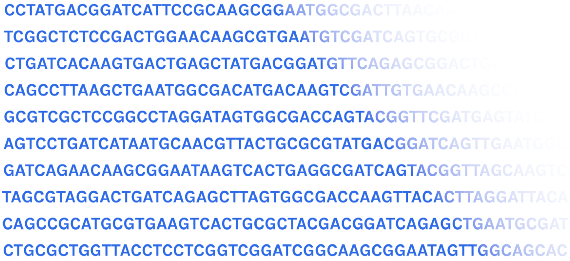
\includegraphics[align=c,height=1in]{figures/dna2.png}
        \hspace*{.2in}
        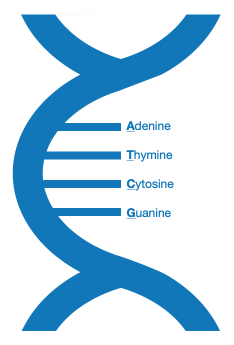
\includegraphics[align=c,height=2in]{figures/dna.png}
    \end{minipage}\hfill
    \caption{DNA and the four bases}
    \label{fig:image:dna}
\end{figure}

In~\cite{heather} Heather and Chain say, ``It is hard to overstate the importance of DNA sequencing to biological research''. Today's researchers use ever-increasing computing resources to process this data faster and in a more complete fashion. String-matching algorithms, mathematical models and other tools have become vital to these research fields, as the size and quantity of data produced by sequencing has also grown. In just the two decades since the completion of the Human Genome Project, current sequencer technology has advanced to the point of being capable of producing as much as a terabyte of data per day~\cite{cabral}.

\subsection{Comparison Bases}
\label{subsec:comparison}

Implementations of the selected algorithms will be developed in five languages: C, C++, Rust, Perl, and Python. Each language's implementations will be evaluated against the others on three bases:

\begin{enumerate}
\item \textbf{Performance}: Overall run-times for each solution will be gathered using existing timer mechanisms. Time-measurements will be somewhat coarse, as overhead operations such as I/O will necessarily be included in the times.
\item \textbf{Energy efficiency}: Energy usage will be measured for each solution using the Running Average Power Limit (RAPL) tools available on Intel processors. RAPL will be outlined in greater detail in section~\ref{subsubsec:rapl}.
\item \textbf{Expressiveness}: Each solution will be measured on several source-level metrics in an effort to evaluate the expressiveness and clarity of the code.
\end{enumerate}

These three bases cover modern concerns in software development: the general performance of an application, the readability/maintainability of the application, and the power consumption of the system running the application. Where the first two criteria are well-known and common, the last has been chosen based on steadily-growing concern over power consumption in the data center industry and in the mobile computing field~\cite{pereira}.


\section{Motivations and Prior Work}
\label{sec:motivations}

This section will discuss some of the motivations that lead to researching this specific topic. Additionally, a range of prior works will be discussed.

\subsection{Programming Languages}

Programming languages have a history. The first commercially-available compiled language was FORTRAN, first appearing in 1956. But there were languages before FORTRAN, languages that were highly specialized and often relied on obscure syntax. Languages evolve and new languages emerge as the applications of computing and the needs of software grow and expand. Some languages, such as C and later versions of Fortran, persist even as new languages intended to replace them fall out of favor and die off. When examining what makes a language successful, it is necessary to look at multiple factors:

\begin{itemize}
\item How well does it perform? How fast are the programs written in the language?
\item What aspects of problem-solving are made easier by the language? What aspects are made harder?
\item How difficult is it to develop software in the language? How difficult is it to maintain?
\end{itemize}

A comparison of languages is not only predicated on their speed but also on readability, expressiveness, and capability. A language must be able to perform, but it must also be understandable. Jokes about the relative readability and maintainability of different languages date back to the APL language if not earlier than that. Setting aside endeavors such as obfuscated code competitions, some languages are simply harder to read than their peers. Perl and Python are often compared in this regard, for example. Perl's syntax relies heavily on use of non-alphabetic symbols (referred to as ``sigils'') in using and referencing variables. Contrast this with Python's comparatively clean syntax, which is closer in style to that of C and other similar languages.

A full treatment on the discipline of programming language design is outside the scope of this writing. Instead, issues of the more aesthetics-oriented language differences will be addressed by examining some static aspects of code, aspects that are completely independent of the running of the programs themselves.

\subsection{Performance, Expressiveness, Energy}

The experiments that will be described in this paper were designed to focus on a trio of aspects of concern to modern software developers: how well the code performs, how easy it is to read and maintain the code, and (more recently) how the code ranks in terms of energy efficiency.

The overall performance of programs is an issue often discussed when languages are compared directly. Languages such as C and C++ offer high performance, while interpreted languages like Perl and Python have comparatively poor performance. And yet, Python holds great popularity in many sub-fields such as data science, machine learning, data visualization, and task automation. It leads to the question: why would a language so much slower would be so popular?

While there are many varied reasons why people developing software like or dislike a given language, certain aspects often rise up in conversations. These aspects include the \textit{friendliness} of the language, the \textit{ease of use} it offers, and the \textit{readability} of the language. Aspects like this are sometimes referred to as the \textit{expressiveness} of a language: the breadth of ideas that can be represented in that language, and the degree to which they can be understood and communicated.

Expressiveness can be a significant factor in language selection and use. In~\cite{berkholz}, Berkholz looks at measuring expressiveness by looking at how many lines of code change in an average version control commit for projects written in a range of languages. He found functional languages such as Lisp and Haskell to be the most expressive, and domain-specific languages to be biased towards high levels of expressiveness.

In addition to performance and expressiveness, the energy usage of software is rapidly becoming more important as data-centers try to reduce carbon footprints and developers target battery-driven devices like mobile phones. In~\cite{pereira}, Pereira et al did an extensive analysis of energy efficiency at the programming language level. Upon seeing the results and the methods used, it became clear that this should be used with the previous two metrics to evaluate a set of languages in even broader terms.

\subsection{The Motivations}

This research began initially as an effort to demonstrate the suitability of the Rust programming language for the bioinformatics field. An exploration of the Rust-Bio project~\cite{rust} led to finding the SeqAn\footnote{SeqAn: \texttt{\url{https://www.seqan.de/}}} project for C++. Further investigation led to an understanding of the ongoing popularity of languages like Perl and Python in this area, as well. It was decided that, rather than focus specifically on Rust and its potential, this effort would instead pursue an understanding of the relative power of a selected set of languages on the metrics described.

It is believed that these three measurements can evaluate the languages with enough clarity that a programmer could make an informed choice as to which would better meet their needs.

\subsection{Prior Work}

Some of the papers that informed this research include:

Rahate and Chandak~\cite{rahate} performed a study focused on algorithm performance similar to what is planned here. From this paper, it was determined that there should be at least five algorithms under consideration and that algorithms such as Knuth-Morris-Pratt~\cite{knuth} would make good candidates.

In~\cite{chen2021string}, Chen and Nguyen describe an approach to string matching over DNA data with $k$ differences. Their technique was based primarily on \textit{edit distance}, and lent ideas to the development of the $k$-gap approximate-matching algorithm that will be described in~\ref{subsec:dfa_gap}.

Neamatollahi et al~\cite{neamatollahi} describe three pattern matching algorithms that are specifically targeted at searches on large DNA sequences. While the first is a more traditional character-based matching algorithm, the second and third take advantage of aspects of the CPU such as word-width to speed up comparisons.

The concept of multiple-pattern-matching for exact matches is explored by Bhuka and Somayajulu in~\cite{bhukya}. Their approach is based on the use of pair indexing for both the sequence and the pattern. This paper gave weight to the idea of multi-pattern matching and led to the decision to take the Aho \& Corasick algorithm~\cite{aho} as one of the evaluation algorithms.

In~\cite{cheng2003approximate}, Cheng et al describe a novel data structure and use it in two new parallel approximate matching algorithms. Ultimately, this was not used directly as the multiple-machine clusters would have greatly increased the complexity of taking energy usage measurements.


\section{Selected Algorithms}
\label{sec:algorithms}

Five algorithms in total were chosen to be used in providing the basis for evaluating the languages under evaluation. Of the five, four are exact-matching algorithms and one is an approximate-matching algorithm. One algorithm matches multiple patterns in a single examination of a sequence, while the remaining algorithms match only single patterns.

In this section, these algorithms are introduced and the first four briefly explained. The fifth algorithm will receive a more in-depth treatment due to it being a new approach.

\subsection{Knuth, Morris, and Pratt}

The Knuth-Morris-Pratt~\cite{knuth.morris.pratt.1977} algorithm is one of the foundational algorithms in the area of string matching and text searching. It is still used in the present day, with implementations as recent as the Rust-Bio project~\cite{rust.bio.2015}. This was chosen primarily for historical significance, but also for ease of implementation.

Knuth-Morris-Pratt is an \textit{exact matching} algorithm, meaning that it matches the desired pattern exactly or not at all. It finds all instances of the pattern within the target string, including overlapping instances, in time linear to the sum of the pattern length and the target length.

Generally when matching, the pattern is aligned with positions in the target string. Shifting is done when a character mismatch is found between an index in the target and the corresponding index in the pattern. Where a na\"{i}ve implementation might shift the pattern by one place after each failed match, resulting in a time complexity approaching O($mn$), the Knuth-Morris-Pratt approach is built on the concept of an auxiliary table (referred to as the ``next'' table) that instructs the matching algorithm on how much to shift the pattern over the target stream. Based on repetition within the pattern itself, the table may call for a shift of the pattern by more than one character for a given mismatch.

The computation of this table is shown in the paper to require O($m$) steps, and the process of matching the pattern to the target takes at most an additional $2n$ steps. This is due to the fact that, at each step of the matching process, only one of the text pointer or the pattern pointer are moved (each of which can only move $n$ times at most). This results in a worst-case run-time bounded by O($m+n$).

As an example, consider a search for the pattern ``CTAGC'' in a sequence that starts with ``CGCCTAGCG''. The first step is to compute the ``next'' table according to the algorithm, shown in figure~\ref{fig:kmp_next}.

\begin{figure}[ht]
\centering
\input{figures/kmp-next}
\caption{Knuth-Morris-Pratt next-table}
\label{fig:kmp_next}
\end{figure}

With the table in hand, the process moves to matching. The matching algorithm goes through the following steps:

\begin{enumerate}
\item $i$ and $j$ both initialize to 0
\item $p_0 = s_0$, so $next$ is not consulted
\item $i$ and $j$ increment, both to 1 and 1
\item $p_1 \neq s_1$, so $i = next[1]$ and becomes 0
\item $p_0 \neq s_1$, so $i = next[0]$ and becomes -1
\item $i$ and $j$ increment, to 0 and 2 respectively
\item $p_0 = s_2$, so $next$ is not consulted
\item $i$ and $j$ increment
\item $p_1 \neq s_3$, so $i = next[1]$ and becomes 0
\item $p_0 = s_3$, so $next$ is not consulted
\item $i$ and $j$ increment
\item $p_i$ continues to match $s_j$ as both variables increment. When $i = 5$, the algorithm detects a match.
\end{enumerate}

Here, the Knuth-Morris-Pratt algorithm has found the match in 10 character comparisons, 5 of which were required to verify the full match.

\subsection{Boyer and Moore}

In the same year that Knuth, Morris and Pratt published their paper, Boyer and Moore published as well~\cite{boyer.moore.1977}. This algorithm is also an exact matching approach, that is based on the research of Knuth, et al. The Boyer-Moore performance improvements are based on searching from the end of the pattern rather than the beginning, and computing two tables to use in optimizing the jumps through the sequence string when mismatches are discovered. This algorithm was chosen as an example of refinement and improvement of another sample algorithm.

Boyer and Moore postulated that, ``more information is gained by matching the pattern from the right than from the left.'' For example: If the target character that corresponds to the current location of the last character from the pattern is not only a mismatch but also does not appear in the pattern at all, the pattern may then be shifted right by its full length. They refer to this algorithm as being ``usually sublinear,'' meaning that when finding the location of the pattern within the target the number of compared characters is usually less than $i+m-1$ (where $m$ is the pattern length and $i$ is the position within the target where the match of the pattern begins).

The first of the two tables is the simplest to compute. It is the size of the alphabet of the pattern and sequence\footnote{In these implementations, to avoid constantly translating the four characters into values between 0 and 3, the alphabet-size was set to 128 for convenience.}, and it tracks the number of positions by which the pattern can be moved down the sequence without additional checking for matches. Boyer and Moore define each entry in this table as being $m$ (the pattern's length) when the character does not appear in the pattern at all, and $m - i$ otherwise (where $i$ is the right-most index within the pattern where the character does occur). Using the same example pattern and sequence as in the previous section, the first table (referred to as $delta_1$ in the paper and $bad\_char$ in the implementations) is shown in figure~\ref{fig:bm_bad_char}. Only the entries for the four characters that appear in patterns are shown.

\begin{figure}[ht]
\centering
\input{figures/bm-bad-char}
\caption{Boyer-Moore $delta_1$ table}
\label{fig:bm_bad_char}
\end{figure}

The second table (referred to as $delta_2$ in the paper and $good\_suffix$ in the implementations) is more complex to calculate, as it first requires calculation of suffixes within the pattern. In the paper, it is described as the distance that the pattern can be slid down in order to align the discovered sub-match (in the target) with the last $m - j$ characters of the pattern (where $j$ is the index within $delta_2$), plus the additional distance that the pointer within the target must be moved so as to restart the matching process at the right end of the pattern. This table is shown in figure~\ref{fig:bm_good_suffix}.

\begin{figure}[ht]
\centering
\input{figures/bm-good-suffix}
\caption{Boyer-Moore $delta_2$ table}
\label{fig:bm_good_suffix}
\end{figure}

When using the two tables to select the amount to shift, it is possible that the $delta_1$ table's value may be negative. Because of this a $max$ operator is applied to the two potential values and the largest possible shift is chosen. With both tables computed, the matching process begins with the pattern aligned to the starting character of the target string. The algorithm then goes through the following steps (where $m$ is the pattern length and $n$ is the sequence length):

\begin{enumerate}
\item $j$ (the pointer within the sequence) initializes to 0
\item $i$ (the pointer within the pattern) is set to $m - 1$ (4)
\item $p_4 \neq s_4$, so the tables are consulted
\item $delta_2(4)$ is 1, and $(delta_1(T) - m + 1 + i)$ = 3
\item $j$ advances by 3
\item $i$ is set to $m - 1$ (4)
\item $p_4 = s_7$, so $i$ is decremented
\item $p_i$ continues to match $s_{i+j}$ until $i$ becomes -1
\item A match is recorded and $j$ advances by $delta_2(0)$, to 7
\end{enumerate}

While the Knuth-Morris-Pratt algorithm had made 10 character comparisons to find the match, Boyer-Moore makes only 6, 5 of which were required to verify the match.

\subsection{Bitap}

The Bitap algorithm (sometimes known as ``Shift-Or'', or ``Shift-Add'') was initially developed by B\'{a}lint D\"{o}m\"{o}lki in 1964. In 1989 it was re-invented by Ricardo Baeza-Yates and Gaston H. Gonnet, and published in~\cite{baeza.yates.gonnet.1992} in 1992. Here, it has been chosen for the distinctive approach when compared to the other algorithms.

In terms of time complexity, the algorithm is on the same level as the previous ones, having a preprocessing time of O($m+\sigma$) (the length of the pattern plus the size of the alphabet) and a running time of O($n$). However, the operations it performs are all bit-oriented: shifts, complements, bitwise-and and bitwise-or. This resulted in this algorithm running significantly faster than either of Knuth-Morris-Pratt or Boyer-Moore on the same input data.

The structure of the algorithm is based on encoding the pattern in a vector of bitmaps. The vector has length equal to the alphabet size, and each element of the vector is a bit-field of width $W$, where $W$ is the size in bits of an unsigned integer. $W$ also limits the length of the pattern in this implementation, though it is possible to implement the algorithm for longer patterns.

The vector is initialized in the preprocessing phase first to an all-1's value in each space, and then modified through a single pass over the pattern. For each character in the pattern, the vector space corresponding to that character has the bit that corresponds to the position in the pattern flipped to 0. The resulting vector fully encodes the pattern. Using the example pattern from the previous two algorithms, imagine that the elements of the vector ($S$) are exactly as wide as the pattern (5 bits) and that there are only the four elements corresponding to the restricted alphabet of the pattern. This is shown in figure~\ref{fig:bitap_s_positions}.

\begin{figure}[ht]
\centering
\input{figures/bitap-s-positions}
\caption{Bitap shift positions vector}
\label{fig:bitap_s_positions}
\end{figure}

During the process of computing the $S$ vector, a ``limit'' value is also calculated: it starts out as 0, and has a number of bits set equal to the full with of the pattern. At the end of the loop that calculates $S$, the value of $limit$ is shifted to the right by one bit, then subject to a bit-complement operation. The result is a value that can be compared to, when determining if a match has been found.

The process of searching for a match begins with a $state$ value of $W$ bit-width, set to all 1's. The target string is read one character at a time. For each iteration of this loop, $state$ is shifted to the left one bit (introducing a 0) and then \texttt{or}'d with the $S$ value of the character under the index. If, after this operation (the ``shift-or''), the value of $state$ is less than the value of $limit$ then a match has been found and will be reported.

\begin{figure}[ht]
\centering
\input{figures/bitap-matching}
\caption{Bitap matching process}
\label{fig:bitap_matching}
\end{figure}

Figure~\ref{fig:bitap_matching} shows the process of matching the example pattern to the same sequence used in previous algorithm examples. The $j$ column indicates the index of the character in the sequence, $s_j$ is the character at $j$, and $S(s_j)$ is the $S$-value for that character. The $state$ column shows the value of that variable at each iteration, while the ``result'' column shows the value of $state$ after the \texttt{or}-operation. Not shown is the $limit$ value, which in this example is \texttt{10000} (16 decimal). On the row where $j = 7$, we see that the high bit of $state$ is a 0 for the first time. This signals a match ($state < limit$), and the matching index is $j - m + 1$, or 3.

In this example the Bitap algorithm has found the match after 8 rounds of the shift-or operation. No direct character-level comparisons were made, nor were any equality comparisons made. The process of finding the match involved only the two bit-level operations and a single ``less-than'' comparison for each iteration of the main loop.

\subsection{Aho and Corasick}

Alfred V. Aho and Margaret J. Corasick published their algorithm for searching multiple patterns at once in 1975~\cite{aho.corasick.1975}. In their algorithm, a finite number of patterns are merged into a single deterministic finite automata (DFA) which can then be applied over any number of target strings. The DFA is capable of finding all locations of all patterns in the set, with overlapping, in a single pass through the target string. This makes the algorithm considerably faster than the others for the simple reason that Aho-Corasick scans each target string once, regardless of the number of patterns. By contrast, each of the previous algorithms would scan the target once per pattern. The choice of this algorithm was driven by an interest in comparing a multi-pattern algorithm to the single-pattern options, and an interest in using a DFA for the matching process.

Aho and Corasick designed the pattern matching machine as a collection of three functions:

\begin{itemize}
\item A ``goto'' function $g$, which maps transitions from one state to the next based on the character being examined
\item A ``failure'' function $f$, which maps a state into another state whenever $g$ reports that there is no transition for the current state and current character
\item An ``output'' function $output$, which maps states to sets of patterns matched at the specific state
\end{itemize}

Construction of these three functions is accomplished through two supporting algorithms. The first fully constructs $g$ and partially computes $output$. The second fully constructs $f$ and completes the computation of $output$. The first algorithm takes only the set of patterns (referred to there as $K$) as input, while the second algorithm takes the resulting $g$ and $output$ from the first as input.

For an example, let $K$ be the list $\left\lbrace ACTG,~CTG,~AAGT \right\rbrace$. Constructing $g$ by the algorithm given in the paper yields the DFA given by the figures~\ref{fig:ac_goto_function} through~\ref{fig:ac_output_function}.

\begin{figure}[ht]
\centering
\input{figures/ac-goto-function}
\caption{Aho-Corasick goto function}
\label{fig:ac_goto_function}
\end{figure}

Starting with figure~\ref{fig:ac_goto_function}, the goto function $g$ provides the finite-state machine that lays out the transitions between states based on the character under consideration. Any state that does not have a transition for a given character is assumed to ``fail'' on that character, which is where the failure function $f$ comes into use. While it is given in the algorithm that there are no failure transitions for state 0, this is made explicit in the figure by including a self-referencing transition for ``G'' and ``T''.

\begin{figure}[ht]
\centering
\input{figures/ac-failure-function}
\caption{Aho-Corasick failure function}
\label{fig:ac_failure_function}
\end{figure}

In figure~\ref{fig:ac_failure_function}, the failure function $f$ shows how the processing of the DFA may jump around to implement a form of back-tracking. State 2 will move to state 5 on a failure transition, reflecting that the character previous to the state (``C'') could instead be the start of matching the ``CTG'' pattern. Because there are no failing transitions in state 0, that state is not represented in the figure.

\begin{figure}[ht]
\centering
\input{figures/ac-output-function}
\caption{Aho-Corasick output function}
\label{fig:ac_output_function}
\end{figure}

In figure~\ref{fig:ac_output_function}, the $output$ function is represented as an indexed array of sets. Most states (including state 0) have the empty set as output. The non-empty sets represent the found patterns by their index in the original list. State 10 has only a value of 2, representing the pattern ``AAGT''. Of note is state 4, whose set includes both the index 0 and the index 1. This reflects the fact that the three characters of pattern 1 overlap the last three characters of pattern 0.

To illustrate the process of this algorithm, consider the target string that begins with the sequence ``AACTG...''. Figure~\ref{fig:ac_progression} shows the progression of states as the pointer advances through the first five characters.

\begin{figure}[ht]
\centering
\input{figures/ac-progression}
\caption{Example of Aho-Corasick state progression}
\label{fig:ac_progression}
\end{figure}

Starting at the 0 state, the first ``A'' moves the DFA to state 1 after which the second ``A'' moves it to state 8. From 8, the character ``C'' is failure transition, so the value of $f(8)$ is read. The value is 1, so the DFA immediately moves to state 1 and looks for a transition on ``C''. It exists, and moves the DFA to states 2, 3 and 4 in turn. Upon reaching state 4 the value of $output(4)$ is checked and found to not be the empty set, so the machine signals a match of the patterns ``ACTG'' and ``CTG''.

\subsection{Approximate Matching with Gaps}

For the fifth and final algorithm in the suite of experiments, it was decided to implement an approximate-matching algorithm. In this case, the algorithm chosen is a new algorithm that takes a different approach to approximate-matching: building a DFA with additional states that allow for measured gaps between the characters of the pattern.

The idea of using a DFA to represent the pattern is inspired primarily by~\cite{aho.corasick.1975} and~\cite{becchi.crowley.2008}. Becchi and Crowley, in particular, address the problem of representing the concept of \textit{counting} states in an extended definition of a finite automata. In their work, they put forward a means of having special states that track the number of times they've been entered in sequence, only allowing exit from the state when the given number (count) of visits is satisfied.

From this, a different type of approximate-matching can be pictured: one that allows for well-defined, finite ``gaps'' between elements of the pattern being matched. Given a value $k$ that is a positive integer, gaps that are up to $k$ characters in length can be tolerated while still regarding the pattern as matching a point in the target sequence. And when $k = 0$, the approach becomes the na\"{i}ve exact-matching approach that is of time-complexity O($mn$).

Current algorithms for approximate matching in DNA sequences use a variety of approaches, such as edit distance. But methods based on edit distance can result in all changes or differences being clumped together as opposed to distributed across the pattern in a more balanced fashion. For example, given the same ``CTAGC'' pattern used for the previous single-pattern algorithms and $k = 3$ this algorithm would allow as many as 12 additions to the pattern in order to match a position in the sequence. Simply allowing an edit distance of 12 in a different algorithm could potentially lead to all 12 additions being between two of the pattern characters. The algorithm described here is designed to prevent such uneven distribution of the gap letters in the matched segment of the sequence.

The basis of the algorithm is the notion that such an approximate match as described here can be expressed in terms of a regular expression that supports the specification of ranges of matches for a given class or symbol in the expression. Such a specification is generally encoded as \texttt{$\lbrace a,b \rbrace$} in an expression, where $a$ and $b$ are integers and $b \geq a$. Most compatible engines support several variant forms of this:

\begin{description}
\item[\texttt{$\lbrace a \rbrace$}:] matches exactly $a$ occurrences
\item[\texttt{$\lbrace a, \rbrace$}:] matches at least $a$ occurrences, with no upper limit
\item[\texttt{$\lbrace ,b \rbrace$}:] matches at most $b$ occurrences, with as few as zero
\item[\texttt{$\lbrace a,b \rbrace$}:] matches at least $a$ occurrences and at most $b$ occurrences
\end{description}

Using the third construct and the ``CTAGC'' pattern, an example regular expression for a value of $k = 3$ could look like:

\begin{center}
\texttt{C.$\lbrace ,3 \rbrace$T.$\lbrace ,3 \rbrace$A.$\lbrace ,3 \rbrace$G.$\lbrace ,3 \rbrace$C}
\end{center}

However, this not quite correct in that the dot ``\texttt{.}'' matches all characters. This is not desirable, as any ``T'' encountered after the initial ``C'' should move to that part of the pattern rather than being subsumed by the dot. Additionally, in a general regular expression engine the dot will match \textit{all} characters, including those not part of the DNA alphabet. Restricting the counting-states to just the alphabet of the problem, and eliminating the target letter from the gap consideration gives us:

\begin{center}
\texttt{C[ACG]$\lbrace ,3 \rbrace$T[CGT]$\lbrace ,3 \rbrace$A[ACT]$\lbrace ,3 \rbrace$G[AGT]$\lbrace ,3 \rbrace$C}
\end{center}

This, given that $k$ is known at the time of the construction, can be readily transformed into a DFA.

As an initial na\"{i}ve approach to the algorithm, the constructed DFA emulates the counting-states by creating $k$ additional states for each of the first $m - 1$ characters of the pattern being searched for. It first creates $m + 1$ states, numbered from 0 to $m$, that represent the start-state and the $m$ characters of the pattern. These are considered the ``trunk'' states. Then for each trunk state from 1 to $m - 1$ (inclusive) the additional states are created as a ``branch'' off of each trunk state. The new states are arranged in such a way as to transition from one to the next on any letter that is \textit{not} the next trunk-state's letter. The last of the branch states will map all non-matching letters to a pre-defined ``failure'' value, indicating that the target letter was not found within a $k$-length gap. This DFA is illustrated in figure~\ref{fig:dfa_dfa}. In this diagram, the branches alternate between left and right of the trunk so as to allow the labels of the transitions to be clearer. The numbering of the states reflects their order of creation, as will be shown later in algorithm~\ref{alg:create_dfa}.

\begin{figure}[ht]
\centering
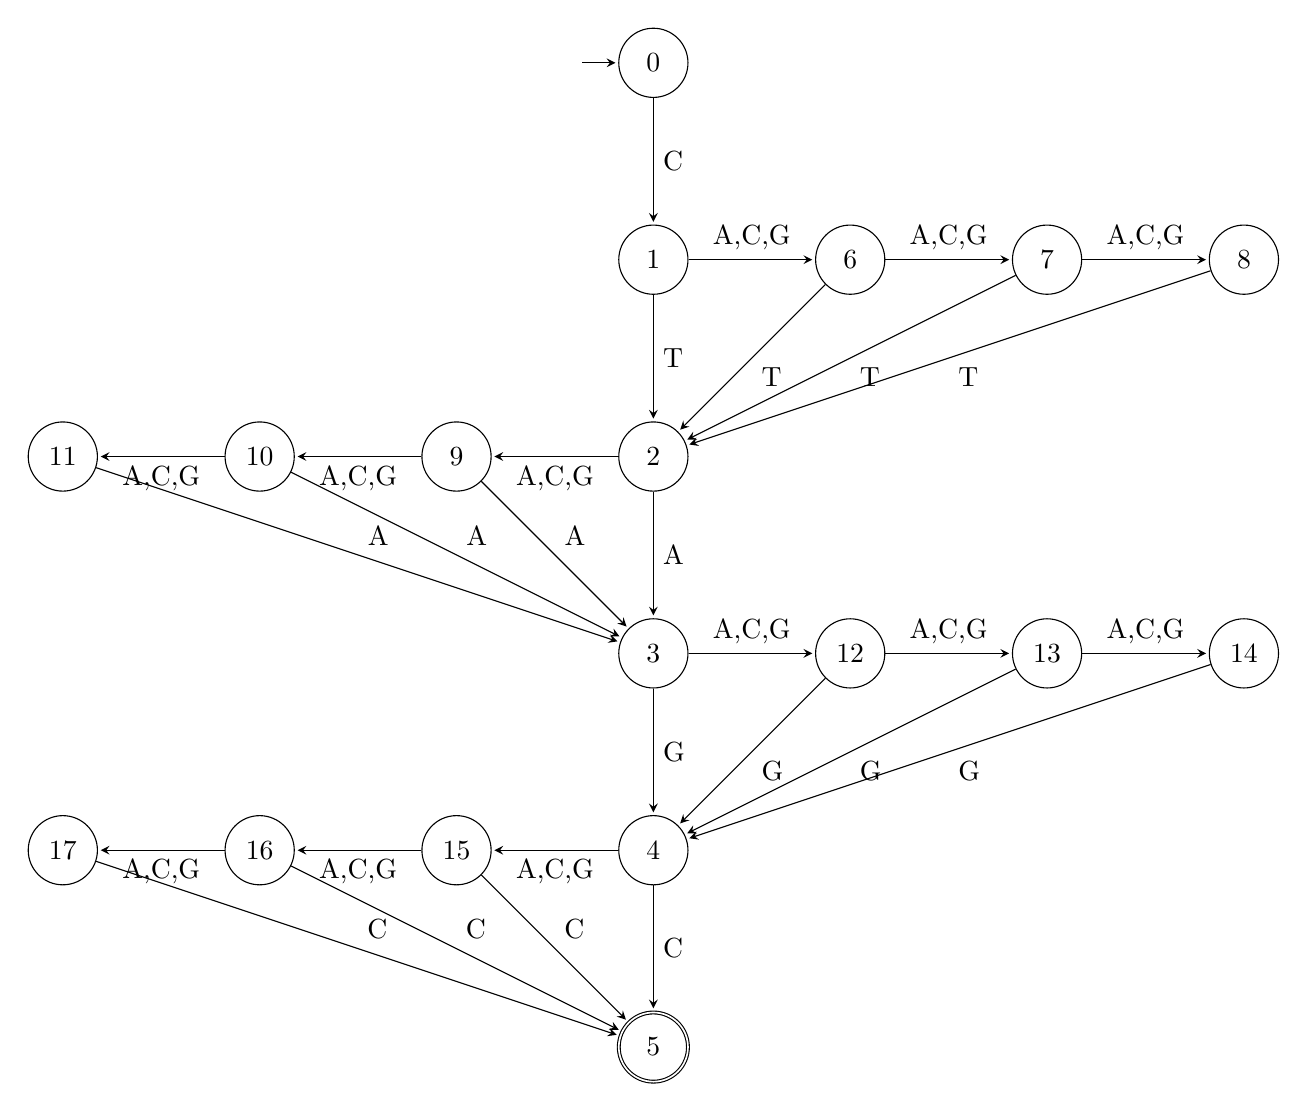
\begin{tikzpicture}[shorten >=1pt,node distance=2.5cm,on grid,auto]
    \node[state,initial]   (s_0)                  {0};
    \node[state]           (s_1)  [below of=s_0]  {1};
    \node[state]           (s_2)  [below of=s_1]  {2};
    \node[state]           (s_3)  [below of=s_2]  {3};
    \node[state]           (s_4)  [below of=s_3]  {4};
    \node[state,accepting] (s_5)  [below of=s_4]  {5};
    \node[state]           (s_6)  [right of=s_1]  {6};
    \node[state]           (s_7)  [right of=s_6]  {7};
    \node[state]           (s_8)  [right of=s_7]  {8};
    \node[state]           (s_9)  [left of=s_2]   {9};
    \node[state]           (s_10) [left of=s_9]   {10};
    \node[state]           (s_11) [left of=s_10]  {11};
    \node[state]           (s_12) [right of=s_3]  {12};
    \node[state]           (s_13) [right of=s_12] {13};
    \node[state]           (s_14) [right of=s_13] {14};
    \node[state]           (s_15) [left of=s_4]   {15};
    \node[state]           (s_16) [left of=s_15]  {16};
    \node[state]           (s_17) [left of=s_16]  {17};

    \path[->]
        (s_0) edge node {C}      (s_1)
        (s_1) edge node {T}      (s_2)
        (s_1) edge node {A,C,G}  (s_6)
        (s_2) edge node {A}      (s_3)
        (s_2) edge node {A,C,G}  (s_9)
        (s_3) edge node {G}      (s_4)
        (s_3) edge node {A,C,G}  (s_12)
        (s_4) edge node {C}      (s_5)
        (s_4) edge node {A,C,G}  (s_15)
        (s_6) edge node {A,C,G}  (s_7)
        (s_6) edge node {T}      (s_2)
        (s_7) edge node {A,C,G}  (s_8)
        (s_7) edge node {T}      (s_2)
        (s_8) edge node {T}      (s_2)
        (s_9) edge node {A,C,G}  (s_10)
        (s_9) edge node {A}      (s_3)
        (s_10) edge node {A,C,G} (s_11)
        (s_10) edge node {A}     (s_3)
        (s_11) edge node {A}     (s_3)
        (s_12) edge node {A,C,G} (s_13)
        (s_12) edge node {G}     (s_4)
        (s_13) edge node {A,C,G} (s_14)
        (s_13) edge node {G}     (s_4)
        (s_14) edge node {G}     (s_4)
        (s_15) edge node {A,C,G} (s_16)
        (s_15) edge node {C}     (s_5)
        (s_16) edge node {A,C,G} (s_17)
        (s_16) edge node {C}     (s_5)
        (s_17) edge node {C}     (s_5);
\end{tikzpicture}

\caption{DFA-Gap finite automaton}
\label{fig:dfa_dfa}
\end{figure}

In this DFA, the number of states needed ($N$) can be easily calculated as a function of $m$ and $k$:

\[N~=~1 + m + k(m - 1)\]

Thus, for a given pattern of length $m$, the size of the DFA grows linearly with $k$.

\subsubsection{Matching with the DFA}

\IncMargin{1em}
\begin{algorithm}[ht]
  \DontPrintSemicolon
  \SetKwInOut{Input}{Input}
  \SetKwInOut{Output}{Output}
  \SetKwFunction{CreateDFA}{CreateDFA}
  \SetKwFunction{Append}{append}
  \SetKwData{Matches}{matches}
  \SetKwData{End}{end}
  \SetKwData{State}{state}
  \SetKwData{Ch}{ch}

  \Input{$P$, the pattern to match ($p_0$ ... $p_{m-1}$)\newline $S$, the sequence to search within ($s_0$ ... $s_{n-1}$)\newline $\Sigma$, the alphabet ($\lbrace~A, C, G, T~\rbrace$)\newline $k$, the maximum gap allowed between characters of $P$}
  \Output{A list of tuples $\left( i, S' \right)$, where $i$ is the starting index of the match and $S'$ is the full matched substring}
  \BlankLine
  \Matches $\leftarrow$ \textit{empty list}\;
  ($q_0$, A, $\delta$) $\leftarrow$ \CreateDFA{$P$,$\Sigma$,$k$}\;
  \End $\leftarrow$ |$S$| - |$P$|\;
  \For{$i \leftarrow 0$ \KwTo \End}{
    \State $\leftarrow q_0$\;
    \Ch $\leftarrow 0$\;
    \While{$\delta(\State,s_{i+\Ch}) \neq$ FAIL}{
      \State $\leftarrow \delta(\State,s_{i+\Ch})$\;
      \Ch $\leftarrow$ $\Ch+1$\;
    }
    \If{\State $\in$ A}{
      S' $\leftarrow$ $S[i~..~(i + \Ch)]$\;
      \Append{\Matches,$(i,~S')$}\;
    }
    \KwRet{\Matches}\;
  }
\caption{FindPatternWithGaps}
\label{alg:find_pattern_with_gaps}
\end{algorithm}
\DecMargin{1em}

\subsubsection{Creation of the DFA}

\IncMargin{1em}
\begin{algorithm}[ht]
  \DontPrintSemicolon
  \SetKwInOut{Input}{Input}
  \SetKwInOut{Output}{Output}
  \SetKwFunction{CreateState}{CreateState}
  \SetKwData{State}{state}
  \SetKwData{NewState}{new\_state}
  \SetKwData{LastState}{last\_state}

  \Input{$P$, the pattern to match ($p_0$ ... $p_{m-1}$)\newline $\Sigma$, the alphabet ($\lbrace~A, C, G, T~\rbrace$)\newline $k$, the maximum gap allowed between characters of $P$}
  \Output{The finite automaton $M = (q_0, A, \delta)$, where $q_0$ is the starting state, $A$ is the set of accepting states ($A \neq \emptyset$), and $\delta$ is the transition function}
  \BlankLine
  $\delta$ $\leftarrow$ \textit{empty list}\;
  \CreateState{$\delta$,0}\;
  $\delta(0, p_0)$ $\leftarrow$ 1\;
  \CreateState{$\delta$,1}\;
  \State $\leftarrow$ 1
  \NewState $\leftarrow$ 1
  \For{$i \leftarrow 1$ \KwTo $m - 1$}{
    \NewState $\leftarrow$ $\NewState+1$\;
    \CreateState{$\delta$,\NewState}\;
    $\delta(\State, p_i)$ $\leftarrow$ \NewState\;
    \LastState $\leftarrow$ \State\;
    \For{$j \leftarrow$ 1 \KwTo $k$}{
      \CreateState{$\delta$,$\NewState + j$}\;
      $\delta(\NewState + j,p_i$) $\leftarrow$ \NewState\;
      $\delta(\LastState,\Sigma - p_i$) $\leftarrow$ $\NewState + j$\;
      \LastState $\leftarrow$ $\NewState + j$\;
    }
    \State $\leftarrow$ \NewState\;
    \NewState $\leftarrow$ $\NewState + k$
  }
  $A$ $\leftarrow$ \State\;
  $q_0$ $\leftarrow$ 0\;
  \KwRet{$(q_0, A, \delta)$}
\caption{CreateDFA}
\label{alg:create_dfa}
\end{algorithm}
\DecMargin{1em}


\section{Details of the Experiments}
\label{sec:experiments}

To gather the desired measurements a range of experiments were executed in the chosen languages (C, C++, Rust, Perl, Python), with the algorithm implementations being run under a ``harness'' application that measured various memory, performance, and energy metrics. Additional tools were used to examine the programs for memory leaks, as well as measure aspects of the source code itself.

\subsection{Definitions and Measurements}

To begin, some concepts will be introduced and terms defined.

\subsubsection{RAPL (Running Average Power Limit)}
\label{subsubsec:rapl}

The \textit{Running Average Power Limit} (RAPL) measurement system was introduced by Intel into their CPU products starting with the Sandybridge family of processors~\cite{khan.et.al.2018}. The system allows measuring energy over several areas:

\begin{description}
\item[Package:] The full (socketed) processor package, which may contain multiple cores.
\item[Power-Plane 0:] The domain that encompasses the combined cores within the package. This reading will cover all cores within the CPU of the package.
\item[Power-Plane 1:] Sometimes referred to as ``uncore'', this domain generally covers the integrated GPU (if present).
\item[DRAM:] The domain for the DRAM memory that the CPU is managing, whose energy usage is separate from the package.
\item[Psys:] The domain that covers the entire system-on-chip energy usage. This would include the package and DRAM values, as well as other system-level energy consumption.
\end{description}

A computer system may have more than one package, and the RAPL interface includes methods for determining the number of packages and gathering the energy readings for each package separately. However, it is not possible to measure a package's energy usage at the level of an individual core.

Reading the RAPL data is done through the \textit{model-specific registers} (MSR) interface, as detailed in~\cite[Chapter~14]{intel.sdm.2022}. The method involves reading several registers to determine the number of packages the system has, then determining the scaling factors for each of time units (expressed in seconds), power units (Watts), and energy units (Joules). The scaling factors are stored in a single register referred to as \texttt{MSR\_RAPL\_POWER\_UNIT}, as groups of bits within the register. Each scaling factor is a 4-bit (5-bit in the case of energy units) value used to compute a fractional floating-point number (where $b$ represents the value of the n-bit factor):

\[S~=~\frac{1}{2^{b}}\]

In the case of the energy units factor, the value of $b$ on the test platform was 01110b (14), and $S~=~61.04~\mu$J.

Obtaining the data during run-time from RAPL required reading from of a series of read-only registers within the MSR and scaling the values obtained by the appropriate value of $S$ for the units. For example, reading the Power-Plane 0 (CPU) energy value uses the \texttt{MSR\_PP0\_ENERGY\_STATUS} register. The value obtained is 64 bits in width, though only the initial 32 bits hold energy data (the high 32 bits are reserved by Intel). The value read is masked to remove any high bits, then multiplied by the energy units scale factor to produce a value in Joules.

An issue with the RAPL system was encountered during runs of the experiments: because the value of the energy registers is 32 bits in size, it wraps around to 0 when the maximum value is reached. This caused occasional anomalous readings in cases where the register would reset between the initial reading and the final reading, resulting in a negative overall value. The program that processed the output from the experiments was adjusted to recognize such values and adjust them by applying a constant value computed as $C~=~S \times 2^{32}$, where $S$ is the scaling factor for that value's type (Package, DRAM, etc.).

Adding the appropriate constant for the type of value that was anomalous dealt with the issue and ensured that all iterations of each algorithm and each language would be usable for the analysis of the results.

\subsubsection{SLOC (Source Lines Of Code)}

The SLOC, or \textit{Source Lines Of Code}, measurement attempts to evaluate the conciseness of the source code to a program. It generally distinguishes between physical lines of text, comments, and actual source lines.

As a metric of code quality or developer productivity, SLOC is not without some controversy. In~\cite{alpernas.2020} the authors point out that measuring lines of code can be very diverse in its execution, and often not clear in its purpose. Nguyen, et al~\cite{nguyen.2007} put forward the basis for an unambiguous standard guide to counting, and describe its use with the support of a configurable counting tool. Here, the purpose of measuring SLOC will be simple: comparison of the implementation of identical algorithms in different languages.

For the purpose of evaluating expressiveness, the SLOC measurements were limited to just the count of actual ``source'' lines as reported by the tool that was eventually chosen for this metric, \texttt{sloc}\footnote{sloc: \texttt{https://github.com/flosse/sloc}}.

\subsubsection{Language Conciseness Through Compression}

In~\cite{bergmans.et.al.2021}, Bergmans, et al describe a technique of measuring the conciseness of programming languages through a process of pre-processing and compressing the source code of a large number of multi-language projects of differing sizes. The higher the compression ratio of the files in a given language, the less concise it is considered to be. The authors hypothesized that this is because a higher compression ratio implies a greater code-redundancy necessary to express the purposes of the program.

Given that none of the experiment source files are of significant length, this metric was applied at the language level, looking at all files for each language in per-language archive files.

\subsubsection{Cyclomatic Complexity}

Thomas McCabe introduced the concept of \textit{cyclomatic complexity} in 1976~\cite{mccabe.1976}. In the most simple terms, it measures the number of paths through a program or function. Sometimes referred to a ``McCabe Complexity'', the measurement is based on measurement of control structures such as conditional (``if'') statements, loops (``for'', ``while'', etc.) and similar means of changing the path of execution through the program or function being measured.

Measuring the complexity in a consistent way is important when comparing different languages. A tool called \texttt{lizard}\footnote{lizard: \texttt{https://github.com/terryyin/lizard}} was used for all languages except Perl, which was not supported by the tool. To gather the metrics for the Perl code a second tool, called \texttt{countperl}\footnote{From the Perl-Metrics-Simple package for Perl, \texttt{https://metacpan.org/dist/Perl-Metrics-Simple}}, was used. It is not clear if the techniques for measuring Perl were completely identical to the techniques used by \texttt{lizard} for the other languages, so this is noted in the results in section~\ref{sec:results}.

\subsubsection{Summary of Metrics}

For each program comprising an experiment, the following data was gathered either dynamically (from executions of the program) or statically (through non-execution analysis of program source code).

\begin{description}
\item[Total Program Run-time:] The complete run-time of the program, as measured by the harness program. Unlike the next metric, this would include program initialization time, the input/output operations of loading the data to be processed, etc. This is measured in floating-point seconds with micro-second resolution.
\item[Algorithm Run-Time:] The time spent specifically within running the algorithm itself over the complete set of test data. This is measured solely on the processing of data, and does not include I/O, set-up of the environment, or post-algorithm steps such as freeing of memory. Also measured in micro-second resolution.
\item[Maximum Memory Usage:] The largest amount of memory allocated for the running program throughout the course of its execution, in megabytes. This represents the largest size to which the program grew during the run.
\item[Power-Plane 0 (CPU) Energy Usage:] The energy consumed by the CPU cores during the execution of the program. Measured over the full lifespan of the program, not just the algorithm itself. Measured in Joules.
\item[DRAM Energy Usage:] The energy consumed by the DRAM during the full lifespan of the program. Measured in Joules.
\item[Full (Package) Energy Usage:] The energy consumed by the full (socketed) package, which includes the CPU cores' energy but not the DRAM energy. Also measured in Joules.
\item[Source Lines Of Code:] The measured lines of code in the implementation of the program, using a tool (\texttt{sloc}) designed to measure these values using consistent standards across the different programming languages.
\item[Cyclomatic Complexity:] The measured complexity of the code, including both the average complexity for the file and specific complexities for those functions that directly correspond to each other across the different implementations.
\end{description}

The Power-Plane 1 (GPU) RAPL values were excluded because the testing machine's package did not have an integrated GPU. Additionally, the Psys values were excluded because they were deemed unnecessary in the context of having the package, CPU and DRAM values.

Independent of the per-program metrics, a measurement of conciseness was made using the compression-based technique described in~\citep{bergmans.et.al.2021}. Using the same tools as were used in that research (\texttt{cloc}\footnote{cloc: \texttt{https://github.com/AlDanial/cloc/}} for removing code comments and \texttt{xz}\footnote{xz: \texttt{https://tukaani.org/xz/}} for data compression), archives of each language's code were compared to each other.

\subsection{Languages}
\label{subsec:languages}

The experiments were performed using five languages. The languages were chosen for their commonalities as well as their differences:

\begin{itemize}
\item Three of the languages (C, C++, Rust) are compiled to machine code and were chosen for performance first and foremost. The remaining two (Perl and Python) are interpreted (``scripting'') languages which are highly regarded for speed of development and rapid prototyping, as well as being popular in bioinformatics computing.
\item Each language is currently in widespread use across different disciplines of software development.
\item The languages showcase differing aspects the approach to memory management, as are detailed below.
\end{itemize}

Each language section includes a sample of the language, implementing the naive (O($mn$)) matching algorithm.

\subsubsection{C}

The C programming language is the oldest and most-established of the languages. Originally designed in the early 1970's by Dennis Ritchie, it remains a very widely-used and influential language since its first appearance in 1972. Since 1989, it has been standardized by both ANSI (the American National Standards Institute) and by the International Organization for Standardization (ISO).

C relies on what is referred to as \textit{manual memory management}, meaning that the programmer is responsible for all allocation and freeing of dynamic memory. This approach can often lead to several major classes of bugs when used incorrectly, such as memory safety issues or memory leaks. Multiple pointers to the same region of memory can become ``dangling pointers'' when one pointer frees the memory without the other pointers being invalidated at the same time. Further attempts to use any of the other pointers can lead to memory corruption or segmentation faults.

Memory management in C is done through a collection of functions in the C standard library, including \texttt{malloc}, \texttt{calloc}, \texttt{realloc}, \texttt{reallocarray}, and \texttt{free}. While \texttt{free} returns allocated memory to the heap, the other functions either allocate memory or change the size of an existing block of allocated memory.

Experiments using the C language were run on three different compiler toolchains: the GNU Compiler Collection (GCC), the LLVM Compiler Infrastructure (LLVM), and the Intel\textregistered~oneAPI Toolkit. Due to the low-level nature of C and the maturity of the compilers, C generally performed the best at each algorithm compared to other languages. Listing~\ref{lst:naive_c} shows a C implementation of the naive algorithm.

\begin{lstlisting}[language=C,caption={C naive implementation},label={lst:naive_c}]
int match(const char *pattern, const char *string, int **matches) {
  int *saved_matches = NULL;
  int found_matches = 0;
  int m = strlen(pattern);
  int n = strlen(string);

  for (int i = 0; i <= n - m; i++) {
    if (!strncmp((const char *)(string + i), pattern, m)) {
      found_matches++;
      saved_matches = realloc(saved_matches,
                              found_matches * sizeof(int));
      saved_matches[found_matches - 1] = i;
    }
  }

  **matches = saved_matches;
  return found_matches;
}
\end{lstlisting}


\subsubsection{C++}

C++ was developed initially as an extension of C, by Bjarne Stroustrup while working at AT\&T Bell Labs. It first appeared in 1985 and was initially standardized in 1998. At first envisioned as ``C with Classes'', the language has been significantly expanded over the years to include many more features while still maintaining low-level memory accessibility. C++ attempts to offer more expressive, concise coding than C, with many of C's memory-management concerns dealt with automatically by class constructors and destructors.

In C++, Stroustrup originated the programming idiom of \textit{resource acquisition is initialization}~\cite{cpp.design.evolution.1994} (RAII). Most dynamic memory is managed via class constructors and destructors, though C++ also supports the \texttt{malloc}-based memory management mechanisms inherited from C.

Experiments using the C++ language were also run on the same three compiler toolchains as C: GCC, LLVM, and Intel. Listing~\ref{lst:naive_cpp} shows the naive algorithm implemented in C++.

\begin{lstlisting}[language=C++,caption={C++ naive implementation},label={lst:naive_cpp}]
std::vector<int> match(std::string pattern, std::string string) {
  std::vector<int> matches;
  int m = pattern.length();
  int n = string.length();

  for (int i = 0; i <= n - m; i++) {
    if (pattern == string.substr(i, m))
      matches.push_back(i);
  }

  return matches;
}
\end{lstlisting}


\subsubsection{Perl}

Perl is a scripting language developed by Larry Wall while working as a programmer at Unisys. The first version, 1.0, was released on December 18, 1987. The current version as of this writing is 5.36.0, released on May 28, 2022.

Perl's reach grew tremendously with the introduction of the World Wide Web's Common Gateway Interface due to its native support for regular expressions and strong text-processing capabilities. Initially developed as a general-purpose scripting language, Perl borrowed features from languages such as C, Awk, Sed, and the \texttt{sh} shell. Perl also offers features generally associated with functional programming, including first-class and higher order functions, lexical closures, garbage collection, and list comprehensions.

Perl is dynamically-typed and multi-paradigm in nature. It supports procedural as well as object-oriented programming styles as well as metaprogramming. Its garbage collection approach to memory management is based on reference counting.

A Perl implementation of the naive algorithm is given in listing~\ref{lst:naive_perl}.

\begin{lstlisting}[language=Perl,caption={Perl naive implementation},label={lst:naive_perl}]
sub match {
    my ($pattern, $string) = @_;

    my $m = length $pattern;
    my $n = length $string;
    my @matches = ();

    for my $i (0 .. ($n - $m)) {
        if ($pattern = substr $string, $i, $m) {
            push @matches, $i;
        }
    }

    return \@matches;
}
\end{lstlisting}


\subsubsection{Python}

Python is another scripting language, developed by Guido van Rossum while at Centrum Wiskunde \& Informatica in the late 1980's and first released as version 0.9.0 in 1991. Like Perl, it is also dynamically-typed and multi-paradigm in its nature. As a language, Python consistently ranks high in user popularity on such measures as the TIOBE Programming Community Index\footnote{TIOBE Index: \texttt{https://www.tiobe.com/tiobe-index/}}.

Python's memory management is a combination of reference counting and a cycle-detecting garbage collector. A Python implementation of the naive algorithm is given in listing~\ref{lst:naive_python}.

\begin{lstlisting}[language=Python,caption={Python naive implementation},label={lst:naive_python}]
def match(pattern, string):
    m = len(pattern)
    n = len(string)
    matches = []

    for i in range(n - m + 1):
        if pattern == string[i:(i + m)]:
            matches.append(i)

    return matches
\end{lstlisting}


\subsubsection{Rust}

Rust is the newest of the languages, having first appeared in 2010. Rust offers a promise of expressiveness equal to or greater than C++, with greater safety in the areas of memory management and ownership. It is a multi-paradigm, general-purpose language that draws from several previous languages including C++, Haskell, and Standard ML. While often referred to as a systems programming language, its usage is spreading rapidly to other areas including to some scientific programming disciplines~\cite{nature.rust.2020}. The language began in 2006 as a personal project of Graydon Hoare, an employee of the Mozilla Corporation, with Mozilla beginning to sponsor the work in 2009 and officially announcing the project in 2010~\cite{asay.2021}. The first pre-alpha numbered version of the compiler was Rust 0.1, which was released in January of 2012. The current (as of this writing) version of Rust is 1.64.0 and was released in September of 2022.

An area where Rust is distinct from other C-based languages is in the way it manages memory and tracks values on the stack and heap. Rust uses an ownership system~\cite[Chapter~4]{programming.rust.2021}, with the ability to specify lifetime information for reference types. There is no automated garbage collection, and resources are managed through the same convention of \textit{resource acquisition is initialization} as in C++, with optional reference counting. Rust's design for memory safety does not permit null pointers, dangling pointers, or data races.

With languages such as C and C++, \textit{data ownership} is handled largely through practice and convention. An instance of a C++ \texttt{std::string} owns the buffer allocated for the storage of the string data. Other variables may be created, though, that point to the same buffer or a single character within it. These other interests in the content of the string buffer have their own responsibility for noticing when the original string object is destroyed and the buffer freed. After such point, the outside interests are each responsible for marking their references as no longer valid.

In contrast, Rust integrates the concept of ownership directly into the language itself. Compile-time checks enforce ownership and report violations. When the owner of a value is ``dropped'' (Rust terminology for freeing) the owned value is dropped as well. While the variables themselves are on the stack, the content is allocated on the heap. Variables own their values, and the complex datatypes (structs, tuples, arrays, and vectors) own their elements.

Listing~\ref{lst:naive_rust} shows the naive algorithm as implemented in Rust. Note that the subroutine is named slightly differently in this case, as \texttt{match} is a keyword in Rust.

\begin{lstlisting}[language=Rust,caption={Rust naive implementation},label={lst:naive_rust}]
fn match_string(pattern: &str, string: &str) -> Vec<usize> {
    let mut matches: Vec<int> = Vec::new();
    let m = pattern.len();
    let n = string.len();

    for i in 0..=(n - m) {
        if pattern == string[i..(i + m)] {
            matches.push(i);
        }
    }

    matches
}
\end{lstlisting}


\subsection{General Implementation of the Algorithms}

Each of the experiment programs providing an algorithm was implemented according to a consistent structure, to better facilitate the direct comparison of the source code across languages. This structure consists of three basic elements:

\begin{itemize}
\item An ``input'' module that encapsulates the loading of sequence, pattern, and answer data
\item A ``runner'' module that provides the controlling loop of the program
\item An ``algorithm'' module that provides the code specific to the algorithm being used as a basis for the experiment
\end{itemize}

The input and runner modules were written once per language and re-used across all five algorithms.

\subsubsection{Input modules}

The input modules allow the main-loop modules (described next) to further abstract the reading of the external data used in each experiment. Data is separated into three files: the \textit{sequences} file contains lines of randomly-generated target strings, the \textit{patterns} file contains the crafted patterns to search for within the sequences, and the \textit{answers} file provides a representation of the correct number of times each pattern should be found in each sequence. This allows the runner modules to verify the results of each invocation of the algorithms being evaluated. The nature of the data and its creation is further detailed in~\ref{subsec:data}.

Each input module defines three routines, one for each of the data files. In most cases, the reading of the pattern files was essentially identical to the sequence files and thus the pattern routine simply calls the sequence routine.

The input modules are the first place in which the distinction in expressiveness and style between the languages becomes apparent. Differences become immediately visible in just the comparison of the C and C++ implementations, where the physical combined length of files (in C and C++, the input modules also required accompanying header files) differs by over 40\% in favor of C++. Python measures as being just over 20\% of the size of the C code.

\subsubsection{Runner modules}

Each runner module utilizes the input module to read in the experiment data and loop over it. In the single-pattern algorithms (which includes the approximate-matching algorithm), this is a nesting of two loops: the outer loop iterates over the set of pattern strings and the inner loop iterates over the set of sequence strings. Each iteration of the loop over the sequence strings triggers one execution of the algorithm being evaluated. In the multi-pattern algorithms, this is a single loop over the set of sequence strings, as the complete set of patterns are pre-processed prior to the loop.

The runner records the time according to the system wall-clock when the algorithm pre-processing begins, and the time when all loops and answer validation has completed. Everything that is not input-related or related to reporting of results is recorded in this span of time. At this point, the runner prints three lines to the standard-output stream. The lines identify the language (including compiler variants for C and C++), the algorithm, and list the time spent in the main loop. The runner is also responsible for handling the arguments passed to the program as well as determining the exit-code of the program (to allow the harness program to discern failing runs from successful runs).

\subsubsection{Algorithm modules}

The algorithm modules are the heart of the experiments. To maintain consistency, each algorithm module defines a minimum of two functions: an initialization routine and the primary algorithm entry point.

The initialization routine is responsible for any pre-processing necessary for the pattern string, and produces a collection of data elements that represent the pattern in the appropriate internal structure. The exact nature and structure of this representation is language-dependent as well as algorithm-dependent.

The algorithm entry point routine is the means by which the each algorithm was applied to the pattern and sequence under consideration. It receives the pattern representation produced by the initialization routine and the sequence representation as parameters, and returns a numerical value indicating how many times the pattern was successfully found within the sequence. In the case of the multi-pattern algorithm implementation, the return value from this routine is a vector of numbers with length equal to the number of patterns.

In addition to these two functions, each algorithm module defines all needed support code for the initialization and entry point. In some cases (such as the C and Rust implementations of the Aho-Corasick algorithm) this included minimal implementations of data structures such as sets and simple queues.

Each algorithm module also provides the language-specific equivalent of a ``main'' function, that function which is treated as the program entry-point by the operating system. Each ``main'' function consists of a single call to the runner function provided by the runner module. The call passes the two algorithm-specific functions as pointers (again, in a language-dependent manner) to the runner, followed by the name of the algorithm and a representation of the command-line arguments.

\subsection{Algorithm Implementation Details}

The different algorithms that were chosen are listed here in the order of their implementation. Each of the algorithms was implemented first in C, as a baseline. These C implementations were then used as templates for the other languages' implementations. In addition to helping to keep the implementations approximately similar and equal, this provided insight into the differences that the features and expressiveness of the different languages made in the development process itself.

\subsubsection{Knuth, Morris, and Pratt}

The C implementation of Knuth-Morris-Pratt was adapted from~\cite[Chapter 7]{handbook.2004}. Of note is the discovery that the sample code quietly takes advantage of C's use of a ``null'' byte at the end of a string to stand in for the sentinel character that the algorithm appends to the pattern string. While this optimization was also applicable to C++ (where strings are represented by instances of the \texttt{std::string} class), each of the three remaining languages were required to manually add a sentinel character to each pattern string prior to computing the corresponding ``next'' table.

This being the first of the algorithms implemented, it is also where the means of passing generic data from the initialization routines to the algorithm routines was developed. The differences in these methods, particularly between the compiled languages, spoke strongly to their relative expressiveness.

In the C implementation it was necessary to use a memory pointer of the type, \texttt{void **}. This defines a dynamic list of dynamic pointers, but provides no information about each individual pointer. It is left to the code to properly type-cast the values from this block of memory. If the program is incorrect (such as getting the order of elements wrong) the resulting typed pointers will likely trigger memory faults when dereferenced. This was also the most-flexible of the compiled solutions and required no difference in implementation between the different algorithms.

In C++ it was initially attempted to reuse the \texttt{void **} approach that had been used in C. This proved to be extremely difficult under the stricter compiler rules, and the decision was made to use the \texttt{std::variant} class instead, which represents a type-safe union in the C++ language. While the same variant type definition could have been used for both the single-pattern and multi-pattern algorithms, it was decided to distinguish them for the sake of readability. The type definitions were made in the file \texttt{run.hpp}, the header-file for the runner module of C++. Unpacking a vector of the variant types brought further type-safety in the form of a generically-typed function \texttt{get<>} in the standard library that was used to extract the values to new objects of the correct type.

Rust had the language features that seemed the most clear and expressive in implementation: enumeration and pattern-matching. In Rust, an enumeration type (\texttt{enum}) can optionally assign data types to the elements of the enumeration. When an enumeration element is instantiated it is provided an instance of that data when applicable. This lead to a system for the Rust programs in which the initialization function for an algorithm created and returned a vector of the enumeration type. The algorithm routines that received these types would extract them from the vector using a pattern-matching\footnote{In the computer language sense, not to be confused with pattern-matching in strings} construct that ensured the types of each individual element of the vector received from the initialization function. The program would raise a run-time exception if the given vector element was not of the expected type. In contrast, Rust required the least-expressive approach to appending the sentinel value onto the pattern string for the sake of creating the ``next'' table.

Given the dynamically-typed nature of data in Perl and Python, both of these implementations were simple lists of values returned without any extra effort at encoding. As with the \texttt{void **} approach the onus was on the program to unpack the elements in the correct order. Trying to use a list or list-reference value as an ordinary scalar value would have caused a run-time exception in either program.

\subsubsection{Boyer and Moore}

The C version of the basic algorithm was drawn from~\cite[Chapter 14]{handbook.2004}. Like Knuth-Morris-Pratt, it requires a character at the end of the pattern for calculating the suffixes table. The C and C++ implementations used the ``null'' string-terminating byte for this while the others added it explicitly.

Starting with Rust in this case, one aspect became very clear in this algorithm's implementation: the need to regularly cast various numerical (particularly integer) types to other types. Because of the larger amount of array-indexing in this algorithm, the number of times an \texttt{i32} (signed 32-bit integer) or \texttt{u32} (unsigned) had to be cast to or from a \texttt{usize} type (an unsigned type used for lengths and indexing) was significant. While this does lead to fewer bugs in the code, at the same time it detracted from the conciseness of the Rust version.

Perl and Python were comparable in their conciseness and logical expression of this algorithm. Python showed an advantage in the form of its native support for iterators as a type and functions such as \texttt{range} that return these iterators. Operations like looping backwards through a series of integers was clearer in the Python code than in the corresponding Perl.

The C and C++ implementations are best compared to each other, as this is another case where the C++ Standard Library classes lead to clearer code. Though there was less difference in code-length, various mechanisms of C++ in areas such as argument-passing meant less overhead and less ambiguity about pointers sent and received.

\subsubsection{Bitap}

The C version of Bitap was taken from~\cite[Chapter 5]{handbook.2004}, where it is referred to as Shift-Or. The design of the algorithm given there is clearly drawn from the Shift-Or algorithm illustrated in~\cite{baeza.yates.gonnet.1992}. The C++ version followed the C very closely with the only changes being the use of the C++ standard classes for strings and vectors. Likewise, the Rust version of this algorithm proved very simple and bore a fair resemblance to the C and C++.

The Perl and Python implementations were also very similar to the compiled versions, with the same exception that each language has arrays as first-class data types. The Python version, however, did have one notable difference: due to Python's integers being of arbitrary size, it was not enough to take the bit-complement of 0 to get a ``full'' bit-field. In Python this resulted in a value of -1, rather than the expected $2^W - 1$ (where $W$ is the word-size used within the algorithm). To force Python to treat these values as unsigned 64-bit, it was necessary to declare a ``mask'' value equal to $2^W - 1$ and apply this to the result of every logical bit-operation performed. This incurred a performance penalty on the Python implementation, making this the only algorithm to be outperformed by its Perl counterpart.

\subsubsection{Aho and Corasick}

For the implementation of this algorithm, no existing code was consulted. Rather, the initial C version was developed directly from the algorithm specification in the paper itself. The C version required the most supporting code, as the algorithm calls for both queue and set data structures. Additionally, the construction of the $g$ and $output$ functions required dynamic re-sizing of lists. It was chosen to avoid this added complexity by generously estimating the size needed for those lists and pre-allocating that amount. Constructing $f$ did not have this problem as the size was known at that point from having created the previous arrays. Both queue and set data structures were implemented with just the minimally-required functionality for each. For the queue, this was the operations \textit{create}, \textit{delete}, \textit{expand} (grow), \textit{enqueue}, \textit{dequeue}, and a test for whether the queue is empty. For the set, these were \textit{insert}, \textit{test-for-membership}, and an implementation of a \textit{union} operation. The set's structure was designed in a such a way that using the C \texttt{calloc} function was sufficient for both creation and initialization, and \texttt{free} was sufficient for deletion and clean-up. That said, these implementations did add to the number of dynamic memory allocations and corresponding releases.

When implementing in C++, the C++ Standard Library was able to provide existing classes for both set and queue implementations, greatly reducing the amount of supporting code in this version. Though C++ vector types can dynamically grow, intermediate experiments found that relying on this for the $g$ and $output$ function construction introduced a slight performance penalty. As such, it was decided to replicate the C approach of estimating their size and pre-allocating. Using C++ features, this also allowed for immediate initialization of the vectors where the C arrays required explicit loops to initialize. In the end, the difference between the two languages' implementations was a factor of almost 2x in SLOC for the C code over the C++ code.

The Perl and Python implementations were both significantly shorter in length than the C or C++, due largely to native support for resizable lists. For the queue data structure, the Python code used the \texttt{collections.deque} class that is part of the Python core. Perl used an ordinary list, as the language provides a built-in keyword for removing from the head of a list in O(1) time. Both languages grew the $g$ and $output$ functions dynamically rather than pre-allocating them. For the implementation of a set data structure, Python provides a \texttt{set} type as a native data type. The Perl version initially used the native associative array type, a common technique for emulating sets in Perl. This proved to be a slight performance penalty, so it was later replaced with a simple list of integers that had duplicates removed as needed.

Lastly, the Rust implementation went through several iterations before reaching its final form. The first version closely followed the C++ version: the use of resizable vectors through the native \texttt{Vec<>} type, and implementations of set and queue from the standard Rust library (\texttt{std::collections::HashSet} and \texttt{std::collections::VecDeque}, respectively). This initial version severely under-performed in comparison to the other two compiled languages. With help from the Rust community, it was determined that the two collection classes were incurring large amounts of overhead. To address this, they were replaced with simple implementations adapted from the C code. As with the Perl and Python versions, the \texttt{Vec<>} type was allowed to handle the dynamic nature of the $g$ and $output$ functions. As with C++, some intermediate experiments were performed that pre-allocated these vectors based on estimates of needed space. But here also it was found that at best the performance remained the same, and in some runs was noticeably worse. As a result, the pre-allocation was removed.

\subsubsection{Approximate Matching by DFA with Gaps}

As this algorithm was new material, it was difficult to anticipate what concerns and issues would arise. Some aspects of each implementation we close in design to the Aho-Corasick code due to the fact that both algorithms are centered around a DFA. All implementations were based on the developed algorithms~\ref{alg:create_dfa} and \ref{alg:find_pattern_with_gaps}, from section~\ref{subsec:dfa_gap}.

As was the case with some of the previous algorithms, the main differences between the C and C++ implementations were in the use of C++ standard library classes in place of manual memory management. The availability of a postfix-increment operator in these languages allowed the two statements of lines 8--9 in algorithm~\ref{alg:find_pattern_with_gaps} to be combined into a single statement. Unlike the Aho-Corasick DFA allocation, this algorithm has a predictable number of states. This made allocation of the DFA much more exact and clean in comparison.

The Rust version of this algorithm is largely identical in structure to the C and C++ versions. In terms of SLOC, it comes in longer than either of those, due primarily to the number of lines used for pattern-matching in the processing of the pattern data structure created by the initialization routine.

The Perl implementation suffered from some readability issues attributable to the ways in which Perl handles slicing an array that has been passed by reference rather than by value. Perl also features a postfix-increment operator, allowing a savings of one line in the SLOC score. In contrast, the Python implementation once again gained conciseness and readability through its clear syntax around iterators and slightly cleaner syntax around treating strings as arrays and applying slicing operations to them.

\subsection{Initial Observations on Complexity}

At this point, some initial observations can be made about the complexity of some of the code. In the code examples given throughout section~\ref{subsec:languages}, all implementations of the naive algorithm had the same cyclomatic complexity value of 3. All also produced the same directed flow graph, shown in figure~\ref{fig:graph-naive}. In this graph, nodes 1 and 6 represent the entry and exit to the function. Node 2 represents the for-loop, and node 3 represents the if-conditional block.

\begin{figure}[ht]
\centering
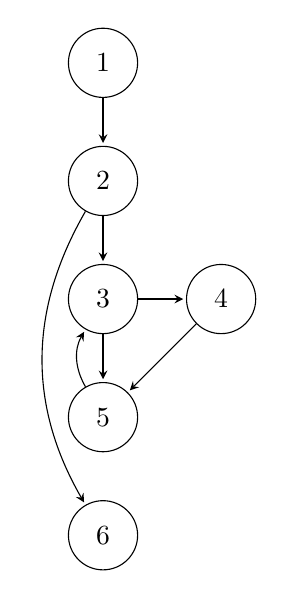
\begin{tikzpicture}[shorten >=1pt,node distance=1.5cm,on grid,auto]
    \node[state] (s_1)                {1};
    \node[state] (s_2) [below of=s_1] {2};
    \node[state] (s_3) [below of=s_2] {3};
    \node[state] (s_4) [right of=s_3] {4};
    \node[state] (s_5) [below of=s_3] {5};
    \node[state] (s_6) [below of=s_5] {6};

    \path[->]
        (s_1) edge             node {} (s_2)
        (s_2) edge             node {} (s_3)
        (s_2) edge[bend right] node {} (s_6)
        (s_3) edge             node {} (s_4)
        (s_3) edge             node {} (s_5)
        (s_4) edge             node {} (s_5)
        (s_5) edge[bend left]  node {} (s_3);
\end{tikzpicture}


\caption{Flow graph of the naive algorithm}
\label{fig:graph-naive}
\end{figure}

Part of the reason for this is that the complexity measurement does not take into account calls to functions that are part of the given language's standard library. In the cases of C and C++, both utilized library functions: \texttt{strncmp} in C and \texttt{substr} in C++. In contrast, the use of \texttt{substr} in Perl is a keyword of the language. Python and Rust skip this entirely by virtue of having array-slicing be a core language feature, along with the ability to compare two slices directly. Had the complexity-measuring tools taken the library calls into account, that would have changed the graph for those languages from one connected component to two, and resulted in a higher complexity score.

Compare this to the \texttt{make\_next\_table} functions defined in the implementations of Knuth-Morris-Pratt. The complexity tool found the Python version to have a score of 6 while the C and C++ versions both scored 5. The reason for the distinction is that C and C++ allocated the array variable \textit{next\_table} prior to the function call and pass it as a parameter. By contrast, in Python \textit{next\_table} was created within the function. The loop used to create it is the source of the extra point of complexity. Figures~\ref{fig:graph-kmp-py} and~\ref{fig:graph-kmp-cpp} illustrate these slightly-different flow graphs. In~\ref{fig:graph-kmp-py}, the extra for-loop represented by states 2 and 3 are where the extra complexity is introduced.

\begin{figure}[ht]
\centering
\begin{minipage}[t]{0.45\textwidth}
\centering
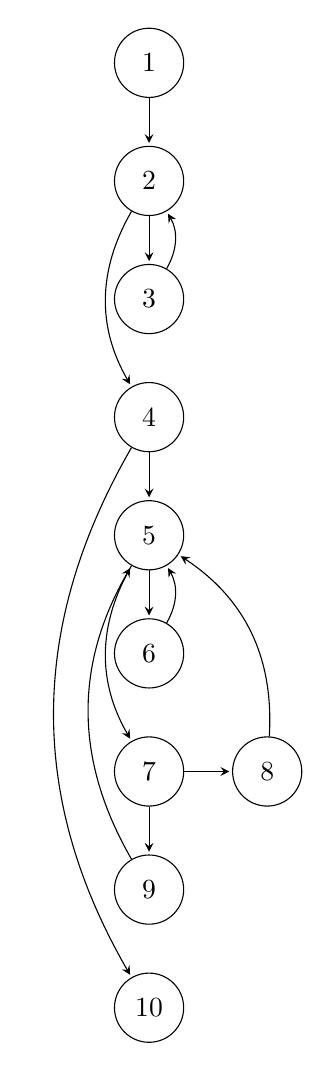
\begin{tikzpicture}[shorten >=1pt,node distance=1.5cm,on grid,auto]
    \node[state] (s_1)                 {1};
    \node[state] (s_2)  [below of=s_1] {2};
    \node[state] (s_3)  [below of=s_2] {3};
    \node[state] (s_4)  [below of=s_3] {4};
    \node[state] (s_5)  [below of=s_4] {5};
    \node[state] (s_6)  [below of=s_5] {6};
    \node[state] (s_7)  [below of=s_6] {7};
    \node[state] (s_8)  [right of=s_7] {8};
    \node[state] (s_9)  [below of=s_7] {9};
    \node[state] (s_10) [below of=s_9] {10};

    \path[->]
        (s_1) edge             node {} (s_2)
        (s_2) edge             node {} (s_3)
        (s_2) edge[bend right] node {} (s_4)
        (s_3) edge[bend right] node {} (s_2)
        (s_4) edge             node {} (s_5)
        (s_4) edge[bend right] node {} (s_10)
        (s_5) edge             node {} (s_6)
        (s_5) edge[bend right] node {} (s_7)
        (s_6) edge[bend right] node {} (s_5)
        (s_7) edge             node {} (s_8)
        (s_7) edge             node {} (s_9)
        (s_8) edge[bend right] node {} (s_5)
        (s_9) edge[bend left]  node {} (s_5);
\end{tikzpicture}


\caption{Flow of the Python \texttt{make\_next\_table} function}
\label{fig:graph-kmp-py}
\end{minipage}\hfill
\begin{minipage}[t]{0.45\textwidth}
\centering
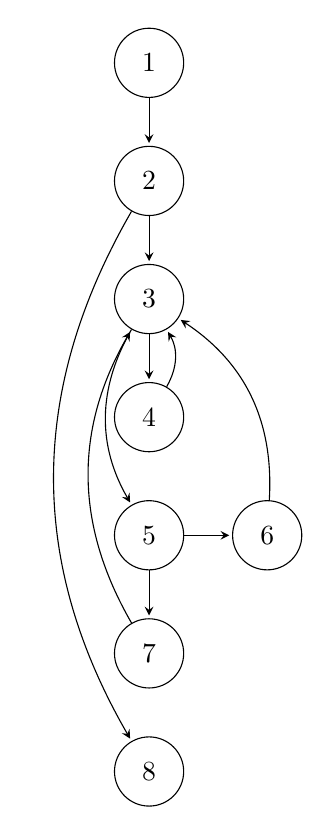
\begin{tikzpicture}[shorten >=1pt,node distance=1.5cm,on grid,auto]
    \node[state] (s_1)                {1};
    \node[state] (s_2) [below of=s_1] {2};
    \node[state] (s_3) [below of=s_2] {3};
    \node[state] (s_4) [below of=s_3] {4};
    \node[state] (s_5) [below of=s_4] {5};
    \node[state] (s_6) [right of=s_5] {6};
    \node[state] (s_7) [below of=s_5] {7};
    \node[state] (s_8) [below of=s_7] {8};

    \path[->]
        (s_1) edge             node {} (s_2)
        (s_2) edge             node {} (s_3)
        (s_2) edge[bend right] node {} (s_8)
        (s_3) edge             node {} (s_4)
        (s_3) edge[bend right] node {} (s_5)
        (s_4) edge[bend right] node {} (s_3)
        (s_5) edge             node {} (s_6)
        (s_5) edge             node {} (s_7)
        (s_6) edge[bend right] node {} (s_3)
        (s_7) edge[bend left]  node {} (s_3);
\end{tikzpicture}


\caption{Flow of the C++ \texttt{make\_next\_table} function}
\label{fig:graph-kmp-cpp}
\end{minipage}
\end{figure}

The resulting complexity of the various implementations is explored in more depth in section~\ref{sec:results}.

\subsection{Optimizations}

Over the course of the development of the experiments in each language, the need became clear for some basic optimizations. In every case, any optimization was applied consistently across all languages. Some examples of optimizations include:

\begin{description}
\item[Data Preprocessing:] While the C and C++ languages were able to seamlessly use individual characters from the strings as array indices, Rust and the scripting languages were not. Based on an assumption that production-targeted code would apply any similar preprocessing, the strings were converted to forms directly usable by the other languages. In the case of Rust, this was a conversion of strings to arrays of unsigned 8-bit integers. In the case of Python, it was a direct mapping of strings (which are already treated as sequences by Python) into the ordinal values of each character. Perl required the most preprocessing, with strings first being converted to arrays of individual characters before being mapped to their ordinal values.
\item[Pattern Preprocessing:] To bring down the running times of the scripting languages' experiments, a mechanism for preprocessing patterns was developed that allowed for each pattern to be processed only once prior to being applied to all sequences. Without this, some instances of the Knuth-Morris-Pratt algorithm (for example) took close to an hour to complete. One the structure of this was established, it was also applied to the compiled languages as well.
\item[Minimizing Type-Casting:] In the case of Rust's strong typing, it was necessary to frequently cast integer values into Rust's \texttt{usize} type for use as array indices. Though this would had little or no effect on run-time, the decision was made in some cases to declare a cast version of the integer value to help in the overall readability of the code.
\item[Compiler Options:] For the three compiled languages, consistent choices of compiler options for optimization were applied. For the C and C++ code, the same options were used for both languages. For the Rust code, the \texttt{cargo} utility was run with an option that instructed the compiler to build optimized code instead of debug-instrumented code. These were not applicable to the Perl and Python code, as both of those are interpreted languages.
\end{description}

All optimization steps were designed to be done inside the timing window of the runner module, and contributed to the reported algorithm run-time.

\subsection{Data Used}
\label{subsec:data}

The data used for the experiments was generated in a random fashion. It was specifically created to emulate basic DNA data, while keeping the size of the data manageable from the perspective of the programs that would be run.

\subsubsection{Method of Generation}

Data generation was handled by a Python script written to allow almost all parameters of the resulting data to be tuned. The script's options included a seed value for the random number generator, which allowed for consistent generation of the data once the parameters were tuned to satisfaction.

Sequence generation was a straightforward process of determining a length from the provided base length and variance values. The standard random number generator provided by Python was then used to draw the sequence of $n$ letters from the set of valid characters.

To ensure that algorithms would be as thoroughly exercised as possible, each candidate pattern was tested before acceptance. The requirement for acceptance was that it match a minimum threshold (0.10\%) of the full set of sequences. Generation of the patterns was done by first selecting the pattern length from the specified range, then extracting a sequence of that length from a random location in a candidate sequence. Candidate sequences were chosen by selecting every $i^{th}$ sequence from the full list (starting with the first sequence), with $i$ being the total number of sequences divided by the total number of patterns being generated.

For the approximate-matching algorithm, the same set of patterns was used since they were already known to meet the minimum-matching criteria. For this algorithm, a $k$ value of 0 would lead to the same set of matches as an exact-matching algorithm would find.

\subsubsection{Shape of the Data Used}

The data set selected for these experiments consisted of the following:

\begin{itemize}
\item 100,000 sequence strings of length ranging from 1,008 to 1,040 characters ($1,024 \pm 16$). The number of patterns and their length was chosen to provide sufficient data to extensively exercise each algorithm implementation, while still fitting within the physical memory of the testing platform.
\item 100 pattern strings of length ranging from 8 to 10 characters ($9 \pm 1$). The length was adjusted several times through command-line parameters to the data-generation utility until a size was found for which the generated patterns would reliably meet the minimum threshold for sequences matched. The matching percentage over the 100 patterns ranged from 0.10\% to 1.62\%, with an average of 0.76\%.
\item A full set of correct counts of each pattern's occurrences in each sequence, as would be found by an exact-matching algorithm. This was established using a backtracking regular expression search for each of the selected patterns over each of the generated sequences. The regular expression was designed to properly include overlapping pattern occurrences.
\item An additional set of answer-files were generated for the approximate-matching algorithm, for values of $k$ ranging from 1 to 5. These, too, were generated using crafted regular expressions that would detect overlapping occurrences of the patterns.
\end{itemize}

A smaller data set was also generated for the purpose of testing and validation of the programs prior to full experiment runs.

The size of the data set was chosen after some preliminary experiments showed this size to be large-enough to rigorously exercise the algorithms while still running in reasonable time overall. This allowed for the experiments to be run repeatedly as the code itself evolved.

\subsection{Testing Platform}

The experiments were run on a dedicated machine running a version of the Linux operating system. The set of installed software was kept minimal to reduce the chance of background processes influencing the readings of general energy usage during the runs of experiments.

\subsubsection{Hardware Specifications}

The machine used for the experiments was an Intel-brand NUC7i5BNH i5-7260U, an ultra-compact device referred to by Intel as a ``Next Unit of Computing'' (NUC). The machine features the following specifications:

\begin{table}[h!]
\begin{center}
\begin{tabular}{|ll|}
\hline
Processor & Intel\textregistered~Core\texttrademark~i5-7260U Processor\\
Processor Base Frequency & 2.20 GHz\\
Max Turbo Frequency & 3.40 GHz\\
Memory Type & DDR4-2133 1.2V SO-DIMM\\
Installed Memory & 8 GB\\
Internal Drive Form Factor & M.2 and 2.5''\\
Installed Storage & 120 GB M.2 SSD\\
\hline
\end{tabular}
\caption{Hardware specifications of the test platform}
\end{center}
\label{table:hardware_specs}
\end{table}

The CPU is dual-core, with hyperthreading cores, for a total of 4 computational cores. This did not come into consideration for the experiments as none of the code was written to be multi-threaded.

\subsubsection{Operating System and Configuration}

The NUC was cleaned of the vendor-installed operating system. Linux was installed on it using the minimal server edition of Ubuntu Linux 22.04.1. All unnecessary packages and software services were either disabled or removed completely.

The development software (see next section) was then installed. This included the Linux version of the ``Homebrew''\footnote{Homebrew: \texttt{https://brew.sh/}} package manager. Homebrew was specifically used to install the latest version of the LLVM Compiler Infrastructure, to allow all experiment code to be compiled directly on the NUC (rather than copying executable files built on a different machine). The Python and Perl interpreters that were used were also provided by Homebrew, as were the majority of the tools used for developing, testing, and evaluating the experiments. The Rust language toolchain was installed and managed using the ``Rustup''\footnote{rustup: \texttt{https://rustup.rs/}} management software. Core software development packages from Ubuntu were also installed at this time.

\subsubsection{Compilers and Other Tools}

Table~\ref{table:tools} lists the primary software tools and packages that were used in the creation and execution of the experiments, with the source from which they were obtained. The double line after the Python details indicates that the remaining tools were used on the development machine only, not on the NUC. These tools were used in the testing and evaluation of the experiments code separately from running experiments on the NUC.

\begin{table}[h!]
\begin{center}
\begin{tabular}{|l|r|l|}
\hline
\textbf{Tool} & \textbf{Version} & \textbf{Source}\\
\hline
GNU Make & 4.3 & Ubuntu 22.04\\
GCC & 11.2.0 & Ubuntu 22.04\\
LLVM & 15.0.3 & Homebrew\\
Intel\textregistered~oneAPI Compiler & 2022.2.0 & Intel\\
Rust & 1.64.0 & Rustup Manager\\
Perl & 5.36.0 & Homebrew\\
Python & 3.10.8 & Homebrew\\
\hline
\hline
Valgrind & 3.20.0 & Homebrew\\
\texttt{sloc} & 0.2.1 & Homebrew\\
\texttt{perf} & 5.15.53 & Ubuntu 22.04\\
\texttt{cloc} & 1.94 & Homebrew \\
\texttt{xz} & 5.2.7 & Homebrew \\
\texttt{lizard} & 1.17.10 & Homebrew \\
\texttt{countperl} & 1.0.1 & Ubuntu 22.04 \\
\hline
\end{tabular}
\caption{List of software tools used}
\label{table:tools}
\end{center}
\end{table}

The tools used for the experiments themselves do include the GNU Make tool, as it was the driver for automating the running of the full range of experiments on a regular basis.

The Valgrind\footnote{Valgrind: \texttt{https://valgrind.org/}} tool was used to identify memory leaks in each of the experiment programs, while \texttt{sloc} was used to measure the Source Lines Of Code metric as part of determining the conciseness and expressiveness of the programs. The \texttt{perf} tool was used to identify performance bottlenecks in the running programs. The tools \texttt{cloc} and \texttt{xz} were used together in the calculation of expressiveness via compression. The \texttt{lizard} tool was used to calculate cyclomatic complexity values for all languages except Perl. Perl complexity was measured using the \texttt{countperl} tool, part of the Perl package \texttt{Perl-Metrics-Simple}, and was installed from the official Ubuntu repositories. Lastly, the Python programming language was used not only for experiments but also to develop the tools which processed and analyzed the data gathered during the running of the experiments, as well as for generating the randomized data that the experiments used to exercise the algorithms.


\section{Results and Analysis}
\label{sec:results}

After the completion of the experiment programs' development, an automation mechanism was developed based on the GNU Make tool. This mechanism allowed for the repeated running of the experiments suite while also providing control over aspects such as the number of repetitions and grouping of the algorithms.

The basis for the mechanism was a series of additional rules added to the already-present ``Makefile'' files that had been developed for the building of each language's set of programs. A single target-rule, ``\texttt{experiments}'', would recursively descend into each language-specific directory and trigger all algorithms in sequence. Each algorithm ran a specified number of times, and in most cases the initial run was discarded. This was to prevent the possibility of the data input files being in the disk device's cache skewing the timing and energy readings with regards to later runs. All non-error output from the experiments was captured by the harness program and streamed to a single text file.

The format chosen for the file of results was YAML\footnote{YAML: \texttt{https://yaml.org/}}, due to the ready availability of parsing libraries. YAML had an advantage over other formats such as CSV (comma-separated values) in that it allowed the flexibility of complex nested data were it to be necessary, while also being emitted in a streaming fashion. This greatly reduced the potential for output to be corrupted between algorithm executions.

\subsection{Results from the Experiments}
\label{subsec:results}

% TODO: Fix date
The automated suite of experiments was run numerous times over the course of this research. The final run from which the analysis and conclusions are drawn is preserved in the same repository on the GitHub platform~\cite{github} as all the other files related to this research. The file of raw data is named ``\texttt{experiments-data-YYYYMMDD.yml}''.

\subsubsection{Scope of the Experiments}

% TODO: Correct num of data points and num of programs
% TODO: Table of runs indexed by language and algorithm
The final run of the experiments generated a total of 1,160 data-points taken from runs of the 25 programs. Table~X shows the number of runs on a per-language, per-algorithm basis.

\subsubsection{Outliers and the Interpreted Languages}

While it was known that the interpreted languages (Python and Perl) would be slower than the compiled languages, the reality of the results was surprising: as will be shown in section~\ref{subsec:perf_comp}, below, the interpreted languages were in some cases more than 150 times slower than the fastest compiled program on the same algorithm.

This discovery required adjusting the automated experiments, to reduce the number of iterations for both interpreted languages. The Knuth-Morris-Pratt, Boyer-Moore, and Bitap algorithms were all reduced to 5 iterations each, for these languages. The Aho-Corasick algorithm ran in a more reasonable length of time and was left at 25 iterations, the same number as were run for the compiled languages.

For the DFA-Gap algorithm, both compiled and interpreted languages had to be reduced in terms of iterations given that approximate-matching algorithms are in general slower than their exact-matching counterparts. The compiled languages ran 10 iterations of this algorithm for values of $k$ ranging from 1 to 5, whereas the interpreted languages were necessarily limited to 3 iterations for the same values of $k$.

\subsection{Performance Comparisons}
\label{subsec:perf_comp}

The following collection of tables show the comparative performance of the languages on each of the algorithms. In each table, the fastest language is listed first with the remaining ones following in order of performance. Run times are scaled by the fastest time. This has the result of showing each slower language's time as a percentage over the fastest.

\subsection{Energy Usage Comparisons}
\label{subsec:energy_comp}

In this section the energy usage results are examined. The following tables show the comparative usage over time (Joules per second) for each algorithm with the same scaling method applied as was used for the performance tables. The tables here use the ``Package'' and ``DRAM'' energy values combined together, divided by total run-time.

\subsection{Expressiveness Comparisons}
\label{subsec:expr_comp}

In comparing expressiveness, it is useful to look at all three of the chosen comparative measures in an aggregated fashion. First, the individual numbers will be examined. As with the previous two bases, tables will show the numbers comparing the languages. Unlike the previous sections, the numbers shown will be for the combined files of all algorithm modules, runner modules, and input modules. For each language the source code was combined in a way that facilitated each of the metrics:

\begin{description}
\item[SLOC:] Total SLOC values for each language's files were combined. In the case of C and C++, this includes relevant lines from the header files for the runner and input modules.
\item[Complexity:] Each file's cyclomatic complexity values were computed on a per-function basis. Any function whose value was exactly 1 was discarded so as to not artificially lower the average complexity for the module. Each module's function-level scores were then averaged, and all modules' averages for a given language were summed together.
\item[Conciseness:] Using a method identical to Bergmans, et al~\cite{bergmans.et.al.2021}, each source code file for a given language was stripped of comments and then archived together using the standard ``\texttt{tar}'' command available on Linux. Each archive file was then compressed with the ``\texttt{xz}'' compression utility and the compression ratio recorded.
\end{description}

\subsection{Combined Bases}
\label{subsec:combined}


\section{Conclusions}
\label{sec:conclusions}

An earlier incarnation of this work was focused on the security benefits of the Rust language. Through the process of research and running of the experiments, the focus changed to that stated in the abstract: finding the best language for bioinformatics based on a balance of three distinct metrics.

And, in the end, that language appears to be Rust.

Over the three bases that will be reviewed below, Rust stood out in two of them. The measure of expressiveness is the only area in which it was not in the top place of the table.

Whether this establishes Rust as the ``best'' language for this purpose cannot be said for certain, for the definition of ``best'' can only be objective up to a point before subjective judgment and feelings begin to influence decisions.

\subsection{Review of Metrics}

In choosing three diverse metrics to measure on, the goal was to provide an environment in which any of the five languages would have the chance to stand out. In this regard the research can be considered successful: each of the five languages managed to be at least as high as the \nth{2} position in at least one metrics table.

\subsubsection{Performance}

Performance was chosen first, and measured most closely, due to the fact that the time a program spends running is one of the most-noticeable features of the program (be that good or bad). Run-time measurement was also the easiest of the metrics to gather, both in terms of total program execution and in wall-clock time specifically spent in the algorithms themselves.

It was in the measuring of performance that it first became clear what a stark difference there would be between the interpreted and compiled languages. One can forget the extent of this gap when working with interpreted languages in-depth for long periods of time. The Perl and Python performance numbers were so large in many cases that they had to be omitted from charts to preserve clarity, even when put to logarithmic scaling.

\subsubsection{Energy Usage}

In regards to energy usage, the only significant barrier to overcome was ensuring that the machine used to run the experiments would be sufficiently isolated so as to have the least amount of interference possible from other running processes. The nature of the RAPL system of measuring power consumption also required that the experiments be run with super-user access levels. This amplified the need for the code to be as safe as possible, even though the testing machine was not made accessible by the general internet.

RAPL posed other challenges to use, such as the previously-mentioned 32-bit limitation in the registers used for tracking the energy usage. But this was overcome, and the RAPL system ended up proving robust-enough to handle measuring programs whose run-times ranged from barely one second to nearly three hours.

\subsubsection{Expressiveness}

Expressiveness was generally the most-challenging of the metrics to measure and evaluate. Even the most concrete, numerical measurements of code such as SLOC and complexity are subject to some debate and dissent. In these aspects of the research, measurement was taken through a range of open-source tools and the results tracked closely with expectation; the interpreted languages showed the strongest scores on the three expressiveness sub-metrics.

However, much of what was measured for this metric was also dependent upon the skill shown in the writing of the programs. Familiarity with the different languages varied, from significant experience in C and Perl to relative newness with regards to Rust. It is not possible to say whether someone more expert in the Rust language, for example, could have implemented the chosen algorithms with more efficiency and better expressiveness metrics.

Additionally, the complexity component of this metric had been cast in some doubt by the inability to use a single tool for all language involved. This was shown in section~\ref{subsec:combined} to have not influenced the final rankings.

\subsection{Real-World Implications}

\subsection{Final Thoughts}

As was said at the start of this section, this research evolved significantly over the span of time it was undertaken.

In the end, the measurements taken and evaluated began to somewhat resemble the concept of a triathlon: it was not necessary for Rust to win every category to have ended up as the recommended solution, the overall winner. Rust did not even achieve notable performance metrics, only being the top-ranked for one of the six algorithms. But Rust's energy performance was very noteworthy, and the performance numbers were steady and reliable across all algorithms leading to Rust leading both of these metrics in the final results.

Late in the process of developing this paper, ZDNet published an article~\cite{tung} by Liam Tung covering a story around the recent recommendations of the National Security Agency that developers consider switching to programming languages that feature greater memory safety. While memory safety was not a primary focus of this research, it is noteworthy that the recommended language is also considered to be the safest in this regard. All of the experiments written in compiled languages were tested with Valgrind and debugged until Valgrind reported no memory-related errors detected\footnote{Perl and Python were not tested with Valgrind, as they are built on bytecode interpreters whose memory-safety is a separate issue.}. Of the compiled languages, only Rust never exhibited any memory errors through Valgrind.

With this, it becomes more understandable why Perkel~\cite{nature} found so many in the sciences turning to Rust as their choice of a performance-oriented language. Though the youngest of the languages evaluated here, Rust has quickly grown to showing great potential for a wide range of applications.

\subsection{Resources}

All source code for all experiment programs, as well as the harness utility described and the Python utilities used for data generation and processing of results, is available on the GitHub platform~\cite{github}.


\singlespacing

\bibliographystyle{plainurl}
\bibliography{thesis}

\onehalfspacing

\appendix

\section{Additional Tables}
\label{sec:extra_tables}

In this appendix is a collection of tables that provide more information on the experiments that were run using the DFA-Gap algorithm and the regular expression variant.

\subsection{DFA-Gap Algorithm Tables}

The following two collections of tables show the full range of results for run-times and for energy usage over time, for the DFA-Gap algorithm on all values of $k$ for which it was run.

\subsubsection{DFA-Gap Run-times}

In table~\ref{table:runtime:dfa_gap:comparative} the different rankings by run-time are shown for the DFA-Gap algorithm. The sixth sub-table, table~\ref{table:runtime:dfa_gap:combined}, shows the score resulting from summing all the values from $k=1$ to $k=5$ and then scoring them.

\begin{table}[!htb]
% Table: Comparative DFA-Gap runtimes sub-tables
% Generated: 2022-11-15 22:08:42.526825
\begin{subtable}{0.49\textwidth}
    \centering
    \caption{$k=1$}
    \label{table:runtime:dfa_gap(1)}
    \begin{tabular}{|l|r|r|}
        %% Caption: $k=1$
        %% Label: table:runtime:dfa_gap(1)
        %% Field(s): ['runtime']
        \hline
        \thead{Language} & \thead{Runtime} & \thead{Score} \\
        \hline
        C (GCC) & 69.49 & 1.0000 \\
        C (LLVM) & 70.13 & 1.0092 \\
        C++ (GCC) & 75.72 & 1.0896 \\
        C++ (LLVM) & 77.95 & 1.1218 \\
        C (Intel) & 81.65 & 1.1750 \\
        C++ (Intel) & 86.37 & 1.2430 \\
        Rust & 104.66 & 1.5061 \\
        Python & 3213.17 & 46.2405 \\
        Perl & 3483.84 & 50.1357 \\
        \hline
    \end{tabular}
\end{subtable}%
\begin{subtable}{0.49\textwidth}
    \centering
    \caption{$k=2$}
    \label{table:runtime:dfa_gap(2)}
    \begin{tabular}{|l|r|r|}
        %% Caption: $k=2$
        %% Label: table:runtime:dfa_gap(2)
        %% Field(s): ['runtime']
        \hline
        \thead{Language} & \thead{Runtime} & \thead{Score} \\
        \hline
        C (GCC) & 83.52 & 1.0000 \\
        C (LLVM) & 89.17 & 1.0677 \\
        C++ (GCC) & 97.42 & 1.1665 \\
        C (Intel) & 99.83 & 1.1953 \\
        C++ (LLVM) & 104.92 & 1.2563 \\
        C++ (Intel) & 108.28 & 1.2965 \\
        Rust & 146.35 & 1.7523 \\
        Python & 4335.62 & 51.9134 \\
        Perl & 4422.84 & 52.9577 \\
        \hline
    \end{tabular}
\end{subtable}
\begin{subtable}{0.49\textwidth}
    \centering
    \caption{$k=3$}
    \label{table:runtime:dfa_gap(3)}
    \begin{tabular}{|l|r|r|}
        %% Caption: $k=3$
        %% Label: table:runtime:dfa_gap(3)
        %% Field(s): ['runtime']
        \hline
        \thead{Language} & \thead{Runtime} & \thead{Score} \\
        \hline
        C (GCC) & 100.45 & 1.0000 \\
        C (LLVM) & 107.97 & 1.0749 \\
        C (Intel) & 116.13 & 1.1561 \\
        C++ (GCC) & 123.25 & 1.2270 \\
        C++ (LLVM) & 133.10 & 1.3250 \\
        C++ (Intel) & 135.04 & 1.3443 \\
        Rust & 177.11 & 1.7632 \\
        Perl & 5647.35 & 56.2209 \\
        Python & 5770.18 & 57.4437 \\
        \hline
    \end{tabular}
\end{subtable}%
\begin{subtable}{0.49\textwidth}
    \centering
    \caption{$k=4$}
    \label{table:runtime:dfa_gap(4)}
    \begin{tabular}{|l|r|r|}
        %% Caption: $k=4$
        %% Label: table:runtime:dfa_gap(4)
        %% Field(s): ['runtime']
        \hline
        \thead{Language} & \thead{Runtime} & \thead{Score} \\
        \hline
        C (GCC) & 119.46 & 1.0000 \\
        C (LLVM) & 130.30 & 1.0907 \\
        C (Intel) & 137.39 & 1.1501 \\
        C++ (GCC) & 151.35 & 1.2670 \\
        C++ (Intel) & 162.98 & 1.3643 \\
        C++ (LLVM) & 164.51 & 1.3771 \\
        Rust & 206.29 & 1.7268 \\
        Perl & 6941.50 & 58.1072 \\
        Python & 7361.39 & 61.6221 \\
        \hline
    \end{tabular}
\end{subtable}
\begin{subtable}{0.49\textwidth}
    \centering
    \caption{$k=5$}
    \label{table:runtime:dfa_gap(5)}
    \begin{tabular}{|l|r|r|}
        %% Caption: $k=5$
        %% Label: table:runtime:dfa_gap(5)
        %% Field(s): ['runtime']
        \hline
        \thead{Language} & \thead{Runtime} & \thead{Score} \\
        \hline
        C (GCC) & 140.60 & 1.0000 \\
        C (LLVM) & 151.92 & 1.0805 \\
        C (Intel) & 155.26 & 1.1043 \\
        C++ (GCC) & 183.42 & 1.3045 \\
        C++ (Intel) & 191.17 & 1.3597 \\
        C++ (LLVM) & 193.67 & 1.3775 \\
        Rust & 235.66 & 1.6761 \\
        Perl & 8354.58 & 59.4222 \\
        Python & 9018.86 & 64.1469 \\
        \hline
    \end{tabular}
\end{subtable}%
\begin{subtable}{0.49\textwidth}
    \centering
    \caption{Combined $k$}
    \label{table:runtime:dfa_gap:combined}
    \begin{tabular}{|l|r|r|}
        \hline
        \thead{Language} & \thead{Runtime} & \thead{Score} \\
        \hline
        C (GCC) & 513.51 & 1.0000 \\
        C (LLVM) & 549.48 & 1.0700 \\
        C (Intel) & 590.26 & 1.1495 \\
        C++ (GCC) & 631.15 & 1.2291 \\
        C++ (LLVM) & 674.15 & 1.3128 \\
        C++ (Intel) & 683.84 & 1.3317 \\
        Rust & 870.06 & 1.6943 \\
        Perl & 28850.11 & 56.1820 \\
        Python & 29699.22 & 57.8356 \\
        \hline
    \end{tabular}
\end{subtable}
\caption{Comparative run-times of DFA-Gap by value of $k$}
\label{table:runtime:dfa_gap:comparative}
\end{table}

This last sub-table acts as an averaging of the results for the different values of $k$. Interesting in these results are that the different compilers for each of C and C++ appear in the same order of ranking for those languages. Rust's combined performance here was over 69\% slower than the fastest, but what is interesting about the performance of Rust is the notable drop in performance for values of $k$ greater than 1. At $k=1$, Rust was only 50.6\% slower than the GCC's C version. But at $k=3$ it was 76.3\%.

Also of interest is how Perl closed the gap on Python as $k$ grew. At $k=4$ they were within 0.07\% of each other and at $k=5$ Perl had outperformed Python.

\subsubsection{DFA-Gap Energy Usage}

Here, in table~\ref{table:energy:dfa_gap:comparative}, the DFA-Gap energy usage rankings are displayed for the range of $k$ values as well as a combined-values score table.

\begin{table}[!htb]
% Table: Comparative DFA-Gap energy sub-tables
% Generated: 2022-11-11 19:03:08.364807
\begin{subtable}{0.33\textwidth}
    \centering
    \caption{$k=1$}
    \label{table:energy:dfa_gap(1)}
    \begin{tabular}{|l|r|}
        %% Caption: $k=1$
        %% Label: table:energy:dfa_gap(1)
        %% Field(s): ['package', 'dram']
        %% Divisor(s): ['total_runtime']
        \hline
        Language & Score \\
        \hline
        Rust & 1.0000 \\
        C (LLVM) & 1.1054 \\
        C (GCC) & 1.1171 \\
        C++ (LLVM) & 1.1189 \\
        C++ (Intel) & 1.1316 \\
        C++ (GCC) & 1.1483 \\
        C (Intel) & 1.1569 \\
        Python & 1.2171 \\
        Perl & 1.3575 \\
        \hline
    \end{tabular}
\end{subtable}%
\begin{subtable}{0.33\textwidth}
    \centering
    \caption{$k=2$}
    \label{table:energy:dfa_gap(2)}
    \begin{tabular}{|l|r|}
        %% Caption: $k=2$
        %% Label: table:energy:dfa_gap(2)
        %% Field(s): ['package', 'dram']
        %% Divisor(s): ['total_runtime']
        \hline
        Language & Score \\
        \hline
        Rust & 1.0000 \\
        C (LLVM) & 1.1359 \\
        C++ (LLVM) & 1.1459 \\
        C++ (Intel) & 1.1718 \\
        C (GCC) & 1.1760 \\
        C (Intel) & 1.1819 \\
        C++ (GCC) & 1.2032 \\
        Python & 1.2666 \\
        Perl & 1.4023 \\
        \hline
    \end{tabular}
\end{subtable}%
\begin{subtable}{0.33\textwidth}
    \centering
    \caption{$k=3$}
    \label{table:energy:dfa_gap(3)}
    \begin{tabular}{|l|r|}
        %% Caption: $k=3$
        %% Label: table:energy:dfa_gap(3)
        %% Field(s): ['package', 'dram']
        %% Divisor(s): ['total_runtime']
        \hline
        Language & Score \\
        \hline
        Rust & 1.0000 \\
        C++ (LLVM) & 1.1603 \\
        C (LLVM) & 1.1812 \\
        C++ (Intel) & 1.2078 \\
        C (Intel) & 1.2231 \\
        C (GCC) & 1.2352 \\
        C++ (GCC) & 1.2497 \\
        Python & 1.3140 \\
        Perl & 1.3897 \\
        \hline
    \end{tabular}
\end{subtable}
\begin{subtable}{0.33\textwidth}
    \centering
    \caption{$k=4$}
    \label{table:energy:dfa_gap(4)}
    \begin{tabular}{|l|r|}
        %% Caption: $k=4$
        %% Label: table:energy:dfa_gap(4)
        %% Field(s): ['package', 'dram']
        %% Divisor(s): ['total_runtime']
        \hline
        Language & Score \\
        \hline
        Rust & 1.0000 \\
        C++ (LLVM) & 1.1515 \\
        C (LLVM) & 1.1977 \\
        C++ (Intel) & 1.2155 \\
        C (Intel) & 1.2287 \\
        C++ (GCC) & 1.2565 \\
        C (GCC) & 1.2735 \\
        Python & 1.3548 \\
        Perl & 1.3595 \\
        \hline
    \end{tabular}
\end{subtable}%
\begin{subtable}{0.33\textwidth}
    \centering
    \caption{$k=5$}
    \label{table:energy:dfa_gap(5)}
    \begin{tabular}{|l|r|}
        %% Caption: $k=5$
        %% Label: table:energy:dfa_gap(5)
        %% Field(s): ['package', 'dram']
        %% Divisor(s): ['total_runtime']
        \hline
        Language & Score \\
        \hline
        Rust & 1.0000 \\
        C++ (LLVM) & 1.1150 \\
        C (LLVM) & 1.1830 \\
        C++ (Intel) & 1.1923 \\
        C (Intel) & 1.2066 \\
        C++ (GCC) & 1.2421 \\
        C (GCC) & 1.2752 \\
        Python & 1.3607 \\
        Perl & 1.3715 \\
        \hline
    \end{tabular}
\end{subtable}%
\begin{subtable}{0.33\textwidth}
    \centering
    \caption{Combined $k$}
    \label{table:energy:dfa_gap:combined}
    \begin{tabular}{|l|r|}
        \hline
        Language & Score \\
        \hline
        Rust & 1.0000 \\
        C++ (LLVM) & 1.1162 \\
        C (LLVM) & 1.1859 \\
        C++ (Intel) & 1.1936 \\
        C (Intel) & 1.2094 \\
        C++ (GCC) & 1.2437 \\
        C (GCC) & 1.2789 \\
        Python & 1.3551 \\
        Perl & 1.3658 \\
        \hline
    \end{tabular}
\end{subtable}
\caption{Comparative energy usage by DFA-Gap by value of $k$}
\label{table:energy:dfa_gap:comparative}
\end{table}

In a result similar to the run-times tables, one language holds the top spot for all values of $k$: Rust. This is an interesting observation, as Rust had consistently scored seventh in run-time performance for these same experiments. This shows that Rust was using energy more efficiently overall, despite needing more time to produce the results. This has already been shown in figure~\ref{fig:graph:total_power_usage}, in section~\ref{subsec:energy_comp}.

\subsection{Regexp-Gap Algorithm Tables}

These tables show the full range of results for run-times and for energy usage over time, for the Regexp-Gap algorithm on all values of $k$ for which it was run.

\subsubsection{Regexp-Gap Run-times}

Table~\ref{table:runtime:regexp_gap:comparative} lays out the run-times of the regular expression variant of the gap algorithm. As with the corresponding collection of tables for the DFA-Gap experiments, a single language dominates the top ranking for all values of $k$. This time, however, the language was Rust. Also of interest is the fact that C++ in all three toolchain variants outperformed all variants of C.

What makes this of such interest is that fact that all three compiled languages were using the same regular expression engine, PCRE2. As PCRE2 is written in C, one might expect the C versions of this experiment to perform the best. Rust and C++ were both using wrappers around the C interface, yet performed better.

\begin{table}[!htb]
% Table: Comparative Regexp runtimes sub-tables
% Generated: 2022-11-09 19:13:24.218899
\begin{subtable}{0.33\textwidth}
    \centering
    \caption{$k=1$}
    \label{table:runtime:regexp(1)}
    \begin{tabular}{|l|r|}
        %% Caption: $k=1$
        %% Label: table:runtime:regexp(1)
        %% Field(s): ['runtime']
        \hline
        Language & Score \\
        \hline
        Rust & 1.0000 \\
        C++ (Intel) & 1.0119 \\
        C++ (GCC) & 1.0157 \\
        C++ (LLVM) & 1.0170 \\
        C (GCC) & 1.0468 \\
        C (Intel) & 1.0475 \\
        C (LLVM) & 1.0503 \\
        Python & 1.4674 \\
        Perl & 3.6431 \\
        \hline
    \end{tabular}
\end{subtable}%
\begin{subtable}{0.33\textwidth}
    \centering
    \caption{$k=2$}
    \label{table:runtime:regexp(2)}
    \begin{tabular}{|l|r|}
        %% Caption: $k=2$
        %% Label: table:runtime:regexp(2)
        %% Field(s): ['runtime']
        \hline
        Language & Score \\
        \hline
        Rust & 1.0000 \\
        C++ (Intel) & 1.0535 \\
        C++ (LLVM) & 1.0578 \\
        C++ (GCC) & 1.0594 \\
        C (Intel) & 1.1136 \\
        C (GCC) & 1.1138 \\
        C (LLVM) & 1.1150 \\
        Python & 1.6380 \\
        Perl & 3.6530 \\
        \hline
    \end{tabular}
\end{subtable}%
\begin{subtable}{0.33\textwidth}
    \centering
    \caption{$k=3$}
    \label{table:runtime:regexp(3)}
    \begin{tabular}{|l|r|}
        %% Caption: $k=3$
        %% Label: table:runtime:regexp(3)
        %% Field(s): ['runtime']
        \hline
        Language & Score \\
        \hline
        Rust & 1.0000 \\
        C++ (LLVM) & 1.1747 \\
        C++ (GCC) & 1.1753 \\
        C++ (Intel) & 1.1794 \\
        C (Intel) & 1.2871 \\
        C (GCC) & 1.2876 \\
        C (LLVM) & 1.2888 \\
        Python & 1.8498 \\
        Perl & 3.7295 \\
        \hline
    \end{tabular}
\end{subtable}
\begin{subtable}{0.33\textwidth}
    \centering
    \caption{$k=4$}
    \label{table:runtime:regexp(4)}
    \begin{tabular}{|l|r|}
        %% Caption: $k=4$
        %% Label: table:runtime:regexp(4)
        %% Field(s): ['runtime']
        \hline
        Language & Score \\
        \hline
        Rust & 1.0000 \\
        C++ (LLVM) & 1.3258 \\
        C++ (GCC) & 1.3316 \\
        C++ (Intel) & 1.3370 \\
        C (Intel) & 1.5162 \\
        C (LLVM) & 1.5170 \\
        C (GCC) & 1.5238 \\
        Python & 2.0552 \\
        Perl & 3.7942 \\
        \hline
    \end{tabular}
\end{subtable}%
\begin{subtable}{0.33\textwidth}
    \centering
    \caption{$k=5$}
    \label{table:runtime:regexp(5)}
    \begin{tabular}{|l|r|}
        %% Caption: $k=5$
        %% Label: table:runtime:regexp(5)
        %% Field(s): ['runtime']
        \hline
        Language & Score \\
        \hline
        Rust & 1.0000 \\
        C++ (LLVM) & 1.4797 \\
        C++ (GCC) & 1.4820 \\
        C++ (Intel) & 1.4865 \\
        C (Intel) & 1.7442 \\
        C (GCC) & 1.7445 \\
        C (LLVM) & 1.7489 \\
        Python & 2.1806 \\
        Perl & 3.8010 \\
        \hline
    \end{tabular}
\end{subtable}%
\begin{subtable}{0.33\textwidth}
    \centering
    \caption{Combined $k$}
    \label{table:runtime:regexp:combined}
    \begin{tabular}{|l|r|}
        \hline
        Language & Score \\
        \hline
        Rust & 1.0000 \\
        C++ (LLVM) & 1.2593 \\
        C++ (GCC) & 1.2616 \\
        C++ (Intel) & 1.2635 \\
        C (Intel) & 1.4144 \\
        C (GCC) & 1.4164 \\
        C (LLVM) & 1.4169 \\
        Python & 1.9108 \\
        Perl & 3.7422 \\
        \hline
    \end{tabular}
\end{subtable}
\caption{Comparative run-times of Regexp-Gap by value of $k$}
\label{table:runtime:regexp_gap:comparative}
\end{table}

Also worthy of note is the relative closeness of the Perl and Python run-times to the compiled language values. This was less surprising, given that both languages' communities have invested time in the performance of their respective regular expression engines. While Perl was still nearly 4x the run-time of Rust in table~\ref{table:runtime:regexp:combined}, that is a great difference over the 56x difference against GCC's C in table~\ref{table:runtime:dfa_gap:combined}.

\subsubsection{Regexp-Gap Energy Usage}

Lastly, table~\ref{table:energy:regexp_gap:comparative} presents the energy usage score for the regular expression variant experiments. Of all the energy comparisons, these are the closest in relation to each other. This would indicate that the regular expression engines of Perl and Python, as well as PCRE2, bore the considerable majority of the work in these experiment runs.

\begin{table}[!htb]
% Table: Comparative Regexp energy sub-tables
% Generated: 2022-11-09 19:13:24.220183
\begin{subtable}{0.33\textwidth}
    \centering
    \caption{$k=1$}
    \label{table:energy:regexp(1)}
    \begin{tabular}{|l|r|}
        %% Caption: $k=1$
        %% Label: table:energy:regexp(1)
        %% Field(s): ['package', 'dram']
        %% Divisor(s): ['total_runtime']
        \hline
        Language & Score \\
        \hline
        Perl & 1.0000 \\
        C (LLVM) & 1.0181 \\
        C (Intel) & 1.0182 \\
        C (GCC) & 1.0204 \\
        C++ (Intel) & 1.0219 \\
        Python & 1.0222 \\
        C++ (LLVM) & 1.0228 \\
        C++ (GCC) & 1.0261 \\
        Rust & 1.0375 \\
        \hline
    \end{tabular}
\end{subtable}%
\begin{subtable}{0.33\textwidth}
    \centering
    \caption{$k=2$}
    \label{table:energy:regexp(2)}
    \begin{tabular}{|l|r|}
        %% Caption: $k=2$
        %% Label: table:energy:regexp(2)
        %% Field(s): ['package', 'dram']
        %% Divisor(s): ['total_runtime']
        \hline
        Language & Score \\
        \hline
        C (Intel) & 1.0000 \\
        Perl & 1.0017 \\
        C (LLVM) & 1.0039 \\
        C (GCC) & 1.0071 \\
        C++ (Intel) & 1.0153 \\
        Python & 1.0154 \\
        C++ (GCC) & 1.0176 \\
        C++ (LLVM) & 1.0178 \\
        Rust & 1.0194 \\
        \hline
    \end{tabular}
\end{subtable}%
\begin{subtable}{0.33\textwidth}
    \centering
    \caption{$k=3$}
    \label{table:energy:regexp(3)}
    \begin{tabular}{|l|r|}
        %% Caption: $k=3$
        %% Label: table:energy:regexp(3)
        %% Field(s): ['package', 'dram']
        %% Divisor(s): ['total_runtime']
        \hline
        Language & Score \\
        \hline
        C (Intel) & 1.0000 \\
        C (GCC) & 1.0055 \\
        C (LLVM) & 1.0094 \\
        C++ (LLVM) & 1.0428 \\
        Perl & 1.0437 \\
        C++ (GCC) & 1.0460 \\
        C++ (Intel) & 1.0473 \\
        Rust & 1.0561 \\
        Python & 1.0604 \\
        \hline
    \end{tabular}
\end{subtable}
\begin{subtable}{0.33\textwidth}
    \centering
    \caption{$k=4$}
    \label{table:energy:regexp(4)}
    \begin{tabular}{|l|r|}
        %% Caption: $k=4$
        %% Label: table:energy:regexp(4)
        %% Field(s): ['package', 'dram']
        %% Divisor(s): ['total_runtime']
        \hline
        Language & Score \\
        \hline
        C (Intel) & 1.0000 \\
        C (LLVM) & 1.0012 \\
        C (GCC) & 1.0047 \\
        Perl & 1.0498 \\
        C++ (GCC) & 1.0544 \\
        C++ (Intel) & 1.0567 \\
        C++ (LLVM) & 1.0569 \\
        Python & 1.0646 \\
        Rust & 1.0647 \\
        \hline
    \end{tabular}
\end{subtable}%
\begin{subtable}{0.33\textwidth}
    \centering
    \caption{$k=5$}
    \label{table:energy:regexp(5)}
    \begin{tabular}{|l|r|}
        %% Caption: $k=5$
        %% Label: table:energy:regexp(5)
        %% Field(s): ['package', 'dram']
        %% Divisor(s): ['total_runtime']
        \hline
        Language & Score \\
        \hline
        C (Intel) & 1.0000 \\
        C (LLVM) & 1.0012 \\
        C (GCC) & 1.0060 \\
        Perl & 1.0696 \\
        C++ (Intel) & 1.0716 \\
        C++ (LLVM) & 1.0722 \\
        C++ (GCC) & 1.0725 \\
        Rust & 1.0751 \\
        Python & 1.0829 \\
        \hline
    \end{tabular}
\end{subtable}%
\begin{subtable}{0.33\textwidth}
    \centering
    \caption{Combined $k$}
    \label{table:energy:regexp:combined}
    \begin{tabular}{|l|r|}
        \hline
        Language & Score \\
        \hline
        C (Intel) & 1.0000 \\
        C (LLVM) & 1.0012 \\
        C (GCC) & 1.0060 \\
        Perl & 1.0687 \\
        C++ (Intel) & 1.0719 \\
        C++ (LLVM) & 1.0724 \\
        C++ (GCC) & 1.0727 \\
        Rust & 1.0763 \\
        Python & 1.0825 \\
        \hline
    \end{tabular}
\end{subtable}
\caption{Comparative energy usage by Regexp-Gap by value of $k$}
\label{table:energy:regexp_gap:comparative}
\end{table}

Noteworthy results here include the presence of Perl in the first position for $k=1$, and never placing lower than fourth. Rust, which had shown strong energy performance for the DFA-Gap experiments, here places last three of the five values of $k$. However, it is almost always within a 1\% difference of the language just ahead of it. This was the case with all of the scoring tables in this grouping; gaps between adjacent scores were rarely more than 1\% in difference and sometimes as little as 0.12\%.

\section{Software Sources}
\label{sec:software_sources}

This paper has referred to a number of software tools and utilities. Some of these are standard features of a UNIX/Linux operating system, but many must be installed from external sources. This appendix is meant to provide sources for these additional tools.

\begin{table}[!htb]
    \begin{tabular}{|l|l|}
        \hline
        \thead{Application or tool} & \thead{Location} \\
        \hline
        Homebrew & \url{https://brew.sh/} \\
        PCRE2 & \url{https://www.pcre.org/} \\
        PCRE2 for Rust & \url{https://crates.io/crates/pcre2} \\
        Rust & \url{https://www.rust-lang.org/} \\
        Rustup & \url{https://rustup.rs/} \\
        Valgrind & \url{https://valgrind.org/} \\
        YAML & \url{https://yaml.org/} \\
        \texttt{cloc} & \url{https://github.com/AlDanial/cloc/} \\
        \texttt{countperl} & \url{https://metacpan.org/dist/Perl-Metrics-Simple} \\
        jPCRE2 & \url{https://github.com/jpcre2/jpcre2} \\
        \texttt{lizard} & \url{https://github.com/terryyin/lizard} \\
        \texttt{rust-code-analysis-cli} & \url{https://github.com/mozilla/rust-code-analysis/} \\
        \texttt{sloc} & \url{https://github.com/flosse/sloc} \\
        \texttt{xz} & \url{https://tukaani.org/xz/} \\
        \hline
    \end{tabular}
    \caption{Sources for the additional software tools used in this research}
    \label{table:software_sources}
\end{table}


\end{document}
